%-------------------------------------------------------%
%      HPCCF Virt. Workshop Presentation CM             %
%-------------------------------------------------------%
\documentclass[english,xcolor=pdftex,dvipsnames,compress,aspectratio=169]{beamer}


%\setbeamertemplate{mini frames}[box]
\usepackage{babel}
\usepackage[utf8]{inputenc}
\usepackage[T1]{fontenc}
\usepackage{amsfonts,amsmath,amssymb}
\usepackage{wrapfig}
\usepackage{pifont}

\usepackage{color,colortbl}
\usepackage{upquote}
% \usepackage{showexpl}
% \lstset{
%     basicstyle=\ttfamily\small,
%     commentstyle=\itshape\ttfamily\small,
%     showspaces=false,
%     showstringspaces=false,
%     breaklines=true,
%     breakautoindent=false,
%     captionpos=t
% }

\definecolor{pblue}{RGB}{45,106,148}
\definecolor{pdarkblue}{RGB}{35,71,100}
\definecolor{plightblue}{RGB}{90,159,212}
\definecolor{pyellow}{RGB}{255,212,59}
\definecolor{pdarkyellow}{RGB}{255,188,41}
\definecolor{orange}{RGB}{255,165,0}
\definecolor{plightyellow}{RGB}{255,232,115}
\definecolor{pdarkgrey}{RGB}{100,100,100}
\definecolor{pgrey}{RGB}{153,153,153}
\definecolor{plightgrey}{RGB}{233,233,233}
\definecolor{plightgrey2}{RGB}{247,247,247}
\definecolor{pnavy}{RGB}{0,0,170}
\definecolor{BrickRed}{RGB}{150,22,11}
\definecolor{BlueViolet}{RGB}{138, 43, 226}
\definecolor{PineGreen}{RGB}{0, 51, 0}
\definecolor{light-gray}{gray}{0.95}

\definecolor{UniRot}{RGB}{193,0,42}
\definecolor{UniDunkelGrau}{RGB}{99,99,99}
\definecolor{UniHellGrau}{RGB}{172,172,172}

\definecolor{UrlColor}{rgb}{0,0.08,0.45}
\definecolor{links}{rgb}{0,0,0}

\usetheme{CambridgeUS} % Pittsburgh, CambridgeUS
\usecolortheme{beaver} %wolverine | crane | beaver | seahorse
\useinnertheme{rounded} 
\useoutertheme{default}
\usefonttheme{default}
%\setbeamercovered{transparent}
\setbeamertemplate{footline}[frame number]
\setbeamersize{text margin left=0.5cm, text margin right=0.5cm}

\setbeamercolor{structure}{fg=UniRot}% to modify  immediately all palettes
\setbeamercolor{title}{fg=UniRot}
\setbeamercolor{title in head/foot}{fg=UniRot}

\setbeamercolor{block title}{bg=UniRot!20,fg=darkred}
\setbeamercolor{block body}{fg=black, bg=plightgrey2}

% \setbeamercolor{block title}{fg=white,bg=orange}
\setbeamercolor{block title alerted}{fg=white,bg=UniRot}
\setbeamercolor{block title example}{fg=white,bg=PineGreen!80}

\graphicspath{{../2019-06-isc/}{../2019-06-isc/fig/}{img/}{../logo/}{images/}}

\usepackage{tikz}
\usetikzlibrary{arrows,shapes,backgrounds,positioning,shadows,decorations,trees,decorations.pathreplacing}


\addtobeamertemplate{footline}{}{%
\begin{tikzpicture}[remember picture,overlay]
\node[anchor=south west,yshift=2pt] at (current page.south west) {
\includegraphics[height=0.8cm]{./images/zdv_logo.png}};
\end{tikzpicture}}

\usepackage[tikz]{bclogo}
\newcommand{\task}[2][Over to you]{\begin{bclogo}[arrondi=0.1,logo=\bcoutil]{#1} #2 \end{bclogo}}
\newcommand{\exercise}[2][ ]{\begin{bclogo}[arrondi=0.1,logo=\bcoutil]{Excercise -- Type: #1}  #2 \end{bclogo}}
\newcommand{\docs}[2][Documentation]{\begin{bclogo}[arrondi=0.1,logo=\bcplume]{#1} #2 \end{bclogo}}
\newcommand{\hint}[2][Hint]{\begin{bclogo}[arrondi=0.1,logo=\bcinfo]{#1} #2 \end{bclogo}}
\newcommand{\warning}[2][Warning]{\begin{bclogo}[arrondi=0.1,logo=\bcattention]{#1} #2 \end{bclogo}}
% ``d/Definition'' is already defined ;-)
\newcommand{\explanation}[2][Definition]{\begin{bclogo}[arrondi=0.1,logo=\bcplume]{#1} #2 \end{bclogo}}
\newcommand{\question}[2][Question]{\begin{bclogo}[arrondi=0.1,logo=\bcquestion]{#1} #2 \end{bclogo}}


\subtitle{HPCCF Virtual Workshop}
\title{\Large Certification Strategy and Contributions}
\author{Christian Meesters (+ HPC Certification Forum)}
\date{2020-05-18}
%\authorURL{https://hpc-certification.org}
%\authorFooter{Christian Meesters \& Julian Kunkel}
%\venue{HPCCF Virtual Workshop}
\institute{HPC Group -- Johannes Gutenberg-University of Mainz}
%\groupLogo{
\includegraphics[width=2.5cm]{hpccf-small}}

\usepackage{multicol}

\usepackage{hhline}

\usepackage{times}

% will decrease the font size for one frame
\newcommand\Fontvi{\fontsize{6}{7.2}\selectfont}

\usepackage{verbatim}
\usepackage{listings}

\lstloadlanguages{Python,bash,C++}
\lstset{showspaces=false,
basicstyle=\small,
showstringspaces=false}


%default python listings:
\lstdefinestyle{Python}
{
  language=Python,
  basicstyle=\small,
  showstringspaces=false,
  stepnumber=5,
  numberstyle=\tiny,
  numbersep=5pt,
  showspaces=false,
  frame=single,
  framerule=0.4pt,
  rulecolor=\color{pgrey},
  backgroundcolor=\color{white},
  stringstyle=\color{BrickRed},
  keywordstyle=\color{BlueViolet}\bfseries,
  commentstyle=\color{PineGreen}\bfseries,
  identifierstyle={},
  emph={[10]self}, emphstyle={[10]\color{pblue}},
  emph={[11]yield}, emphstyle={[11]\color{pblue}},
}

%default python listings:
\lstdefinestyle{C++}
{
  language=C++,
  basicstyle=\small,
  showstringspaces=false,
  stepnumber=5,
  numberstyle=\tiny,
  numbersep=5pt,
  showspaces=false,
  frame=single,
  framerule=0.4pt,
  rulecolor=\color{pgrey},
  backgroundcolor=\color{white},
  stringstyle=\color{BrickRed},
  keywordstyle=\color{BlueViolet}\bfseries,
  commentstyle=\color{PineGreen}\bfseries,
  identifierstyle={},
  emph={[10]self}, emphstyle={[10]\color{pblue}},
  emph={[11]yield}, emphstyle={[11]\color{pblue}},
}

\newcommand{\CC}{C\nolinebreak\hspace{-.05em}\raisebox{1ex}{\tiny\bf +}\nolinebreak\hspace{-.10em}\raisebox{1ex}{\tiny\bf +}}

%default shell listings:
\lstdefinestyle{Shell}
{
  language=Bash,
  basicstyle=\ttfamily\small,
  showstringspaces=false,
  frame=single,
  framerule=0.4pt,
  rulecolor=\color{pgrey},
  backgroundcolor=\color{plightgrey2},
  stringstyle=\color{BrickRed},
  keywordstyle=\color{BlueViolet},
  commentstyle=\color{PineGreen}\bfseries,
  identifierstyle=\color{black},
  emph={[10]\$,>>>}, emphstyle={[10]\color{pblue}},
  moredelim=**[is][\bfseries\color{red}]{@}{@}
}

%default plain listings (e.g. for config files):
\lstdefinestyle{Plain}
{ 
  stepnumber=5,
  numberstyle=\tiny,
  numbersep=5pt,
  language=Bash,
  basicstyle=\ttfamily\small,
  showstringspaces=false,
  frame=single,
  framerule=0.4pt,
  rulecolor=\color{pgrey},
  backgroundcolor=\color{plightgrey2},
  stringstyle=\color{black},
  keywordstyle=\color{black},
  commentstyle=\color{blue}\bfseries,
  identifierstyle=\color{black},
  emph={[10]\$,>>>}, emphstyle={[10]\color{pblue}}
}
\lstdefinelanguage{XML}
{
  frame=single,
  framerule=0.4pt,
  rulecolor=\color{pgrey},
  backgroundcolor=\color{plightgrey2},
  stringstyle=\color{black},
  keywordstyle=\color{black},
  commentstyle=\color{blue}\bfseries,
  identifierstyle=\color{black},
  emph={[10]\$,>>>}, emphstyle={[10]\color{pblue}}
  morestring=[b]",
  morestring=[s]{>}{<},
  morecomment=[s]{<?}{?>},
  morekeywords={xmlns,version,type}% list your attributes here
}

\newcommand{\bibtex}{\textsc{Bib}\TeX}

%%% https://tex.stackexchange.com/questions/99316/symbol-for-external-links
\newcommand{\LinkSymbol}{%
  \tikz[x=1.2ex, y=1.2ex, baseline=-0.05ex]{% 
    \begin{scope}[x=1ex, y=1ex]
      \clip (-0.1,-0.1) 
      --++ (-0, 1.2) 
      --++ (0.6, 0) 
      --++ (0, -0.6) 
      --++ (0.6, 0) 
      --++ (0, -1);
      \path[draw, 
      line width = 0.5, 
      rounded corners=0.5] 
      (0,0) rectangle (1,1);
    \end{scope}
    \path[draw, line width = 0.5] (0.5, 0.5) 
    -- (1, 1);
    \path[draw, line width = 0.5] (0.6, 1) 
    -- (1, 1) -- (1, 0.6);
  }
}
\newcommand{\lhref}[2]{\href{#1}{#2\,\LinkSymbol}}

%%%% shortcuts for uniform appearance of common strings %%%%
\newcommand{\slurm}{\textsc{slurm}~}
\makeatletter
\newcommand{\rmnum}[1]{\romannumeral #1}
\newcommand{\Rmnum}[1]{\expandafter\@slowromancap\romannumeral #1@}
\makeatother
\usepackage{xspace}
\newcommand{\mogon}{\textsc{mogon}\xspace}
\newcommand{\mogonI}{\textsc{mogon}\,\Rmnum{1}\xspace}
\newcommand{\mogonII}{\textsc{mogon}\,\Rmnum{2}\xspace}

\setcounter{tocdepth}{1}


%%%%%%%%%%%%%%%%%%%%%%%%%%%%%%%%%%%%%%%%%%%%%%%%%%%%%%%%%%%%%%%%%%%%%%%%%%%%%%%%
%%%%%%%%%%%%%%%%%%%%%%%%%%%%%%%%%%%%%%%%%%%%%%%%%%%%%%%%%%%%%%%%%%%%%%%%%%%%%%%%
\begin{document}
%%%%%%%%%%%%%%%%%%%%%%%%%%%%%%%%%%%%%%%%%%%%%%%%%%%%%%%%%%%%%%%%%%%%%%%%%%%%%%%%
%%%%%%%%%%%%%%%%%%%%%%%%%%%%%%%%%%%%%%%%%%%%%%%%%%%%%%%%%%%%%%%%%%%%%%%%%%%%%%%%

% Passe captions an
\setbeamertemplate{caption}{\insertcaption}
% \setbeamerfont{caption}{size=\scriptsize}
\setlength\abovecaptionskip{-2.5pt}
\setlength\belowcaptionskip{0pt}



% For every picture that defines or uses external nodes, you'll have to
% apply the 'remember picture' style. To avoid some typing, we'll apply
% the style to all pictures.
\tikzstyle{every picture}+=[remember picture]
\tikzstyle{na} = [baseline=-.5ex]

%%%%%%%%%%%%%%%%%%%%%%%%%%%%%%%%%%%%%%%%%%%%%%%%%%%%%%%%%%%%%%%%%%%%%%%%%%%%%%%% 
\begin{frame}[plain] % plain erzeugt Titelseite ohne Kopf- und Fußzeile
  \titlepage
\end{frame}

%%%%%%%%%%%%%%%%%%%%%%%%%%%%%%%%%%%%%%%%%%%%%%%%%%%%%%%%%%%%%%%%%%%%%%%%%%%%%%%%
\section[Certification Strategy]{strategy}

%%%%%%%%%%%%%%%%%%%%%%%%%%%%%%%%%%%%%%%%%%%%%%%%%%%%%%%%%%%%%%%%%%%%%%%%%%%%%%%%
\subsection[What's in for Users]{Users}


%%%%%%%%%%%%%%%%%%%%%%%%%%%%%%%%%%%%%%%%%%%%%%%%%%%%%%%%%%%%%%%%%%%%%%%%%%%%%%%%
\begin{frame}
  \frametitle{How the Site Manager looks on HPC Education}
  \centering
  {\bcattention \bf \large Exaggeration Warning \bcattention}
  \begin{columns}
   \begin{column}{0.6\textwidth}
    \centering
    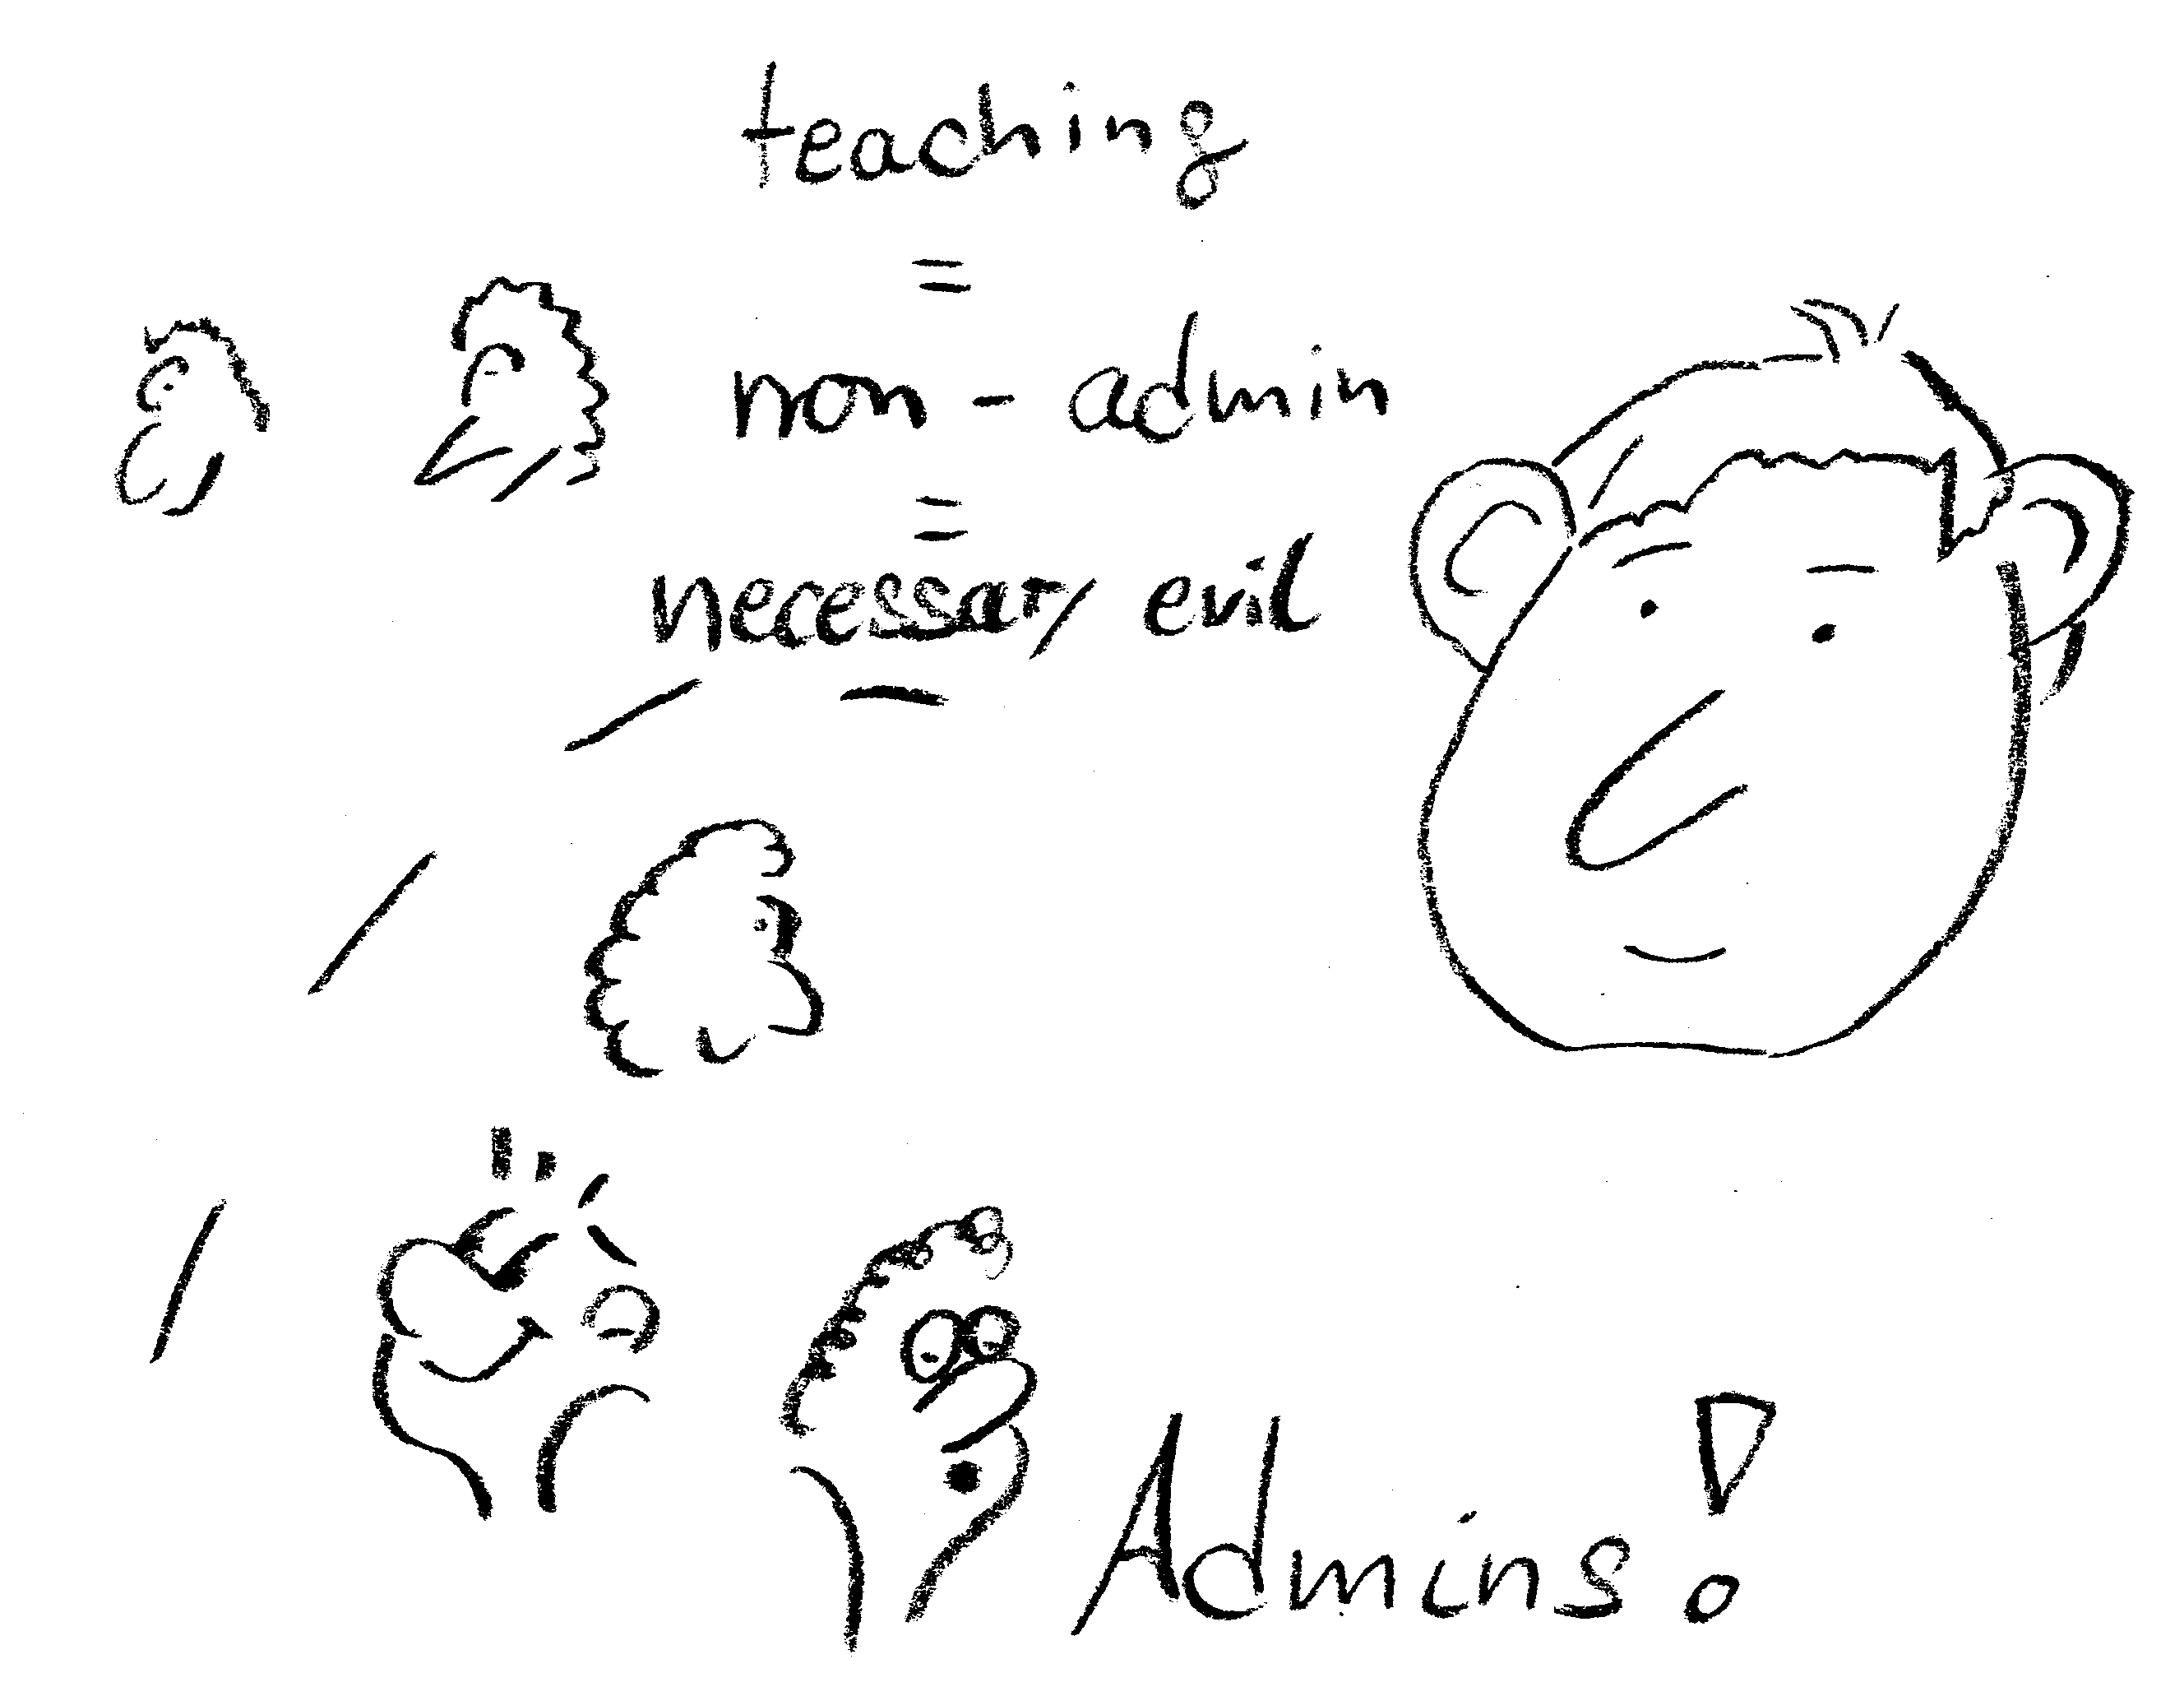
\includegraphics[width=0.8\textwidth]{images/runner}
   \end{column}
   \begin{column}{0.4\textwidth}
    \pause
    \begin{itemize}[<+->]
     \item ressources are always limited
     \item teaching ressources even more
     \item integration into HPCCF might offer more (still needed) courses
    \end{itemize}
   \end{column}
  \end{columns}
\end{frame}

%%%%%%%%%%%%%%%%%%%%%%%%%%%%%%%%%%%%%%%%%%%%%%%%%%%%%%%%%%%%%%%%%%%%%%%%%%%%%%%%
\begin{frame}
  \frametitle{HPCCF Adoption by Sites}
  \begin{columns}
   \begin{column}{0.5\textwidth}
    \centering
    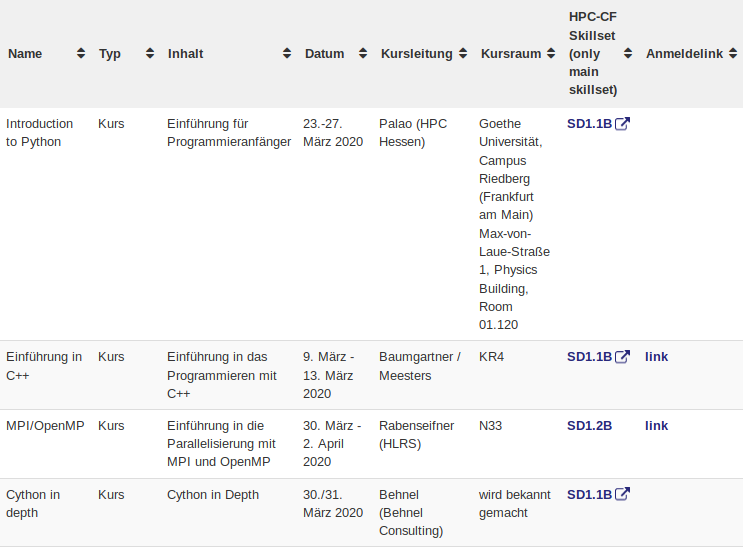
\includegraphics[width=0.8\textwidth]{images/linking_skills}\\
    \lhref{https://hpc.uni-mainz.de/kurse-und-workshops/\#bersicht}{Mainz course overview}
   \end{column}
   \begin{column}{0.5\textwidth}
     Assigning HPCCF skill labels to courses is no of cost, yet they are an asset for participating sites:
     \begin{itemize}
      \item enhanced transparency of own course portfolio
      \item own portfolio can be complemented by linking to courses nearby $\curvearrowright$ (for smaller sites) not so thin anymore
      \item with transparency a plus for users
      \item with HPCCF certificates new users may have some HPC experience other than ``submitted a job'' once
     \end{itemize}
   \end{column}
  \end{columns}
\end{frame}


%%%%%%%%%%%%%%%%%%%%%%%%%%%%%%%%%%%%%%%%%%%%%%%%%%%%%%%%%%%%%%%%%%%%%%%%%%%%%%%%
\begin{frame}
  \frametitle{How Joe User looks on HPC}
  \centering
  {\bcattention \bf \large Exaggeration Warning \bcattention}
  \begin{columns}
    \begin{column}{.5\textwidth}
     \centering
     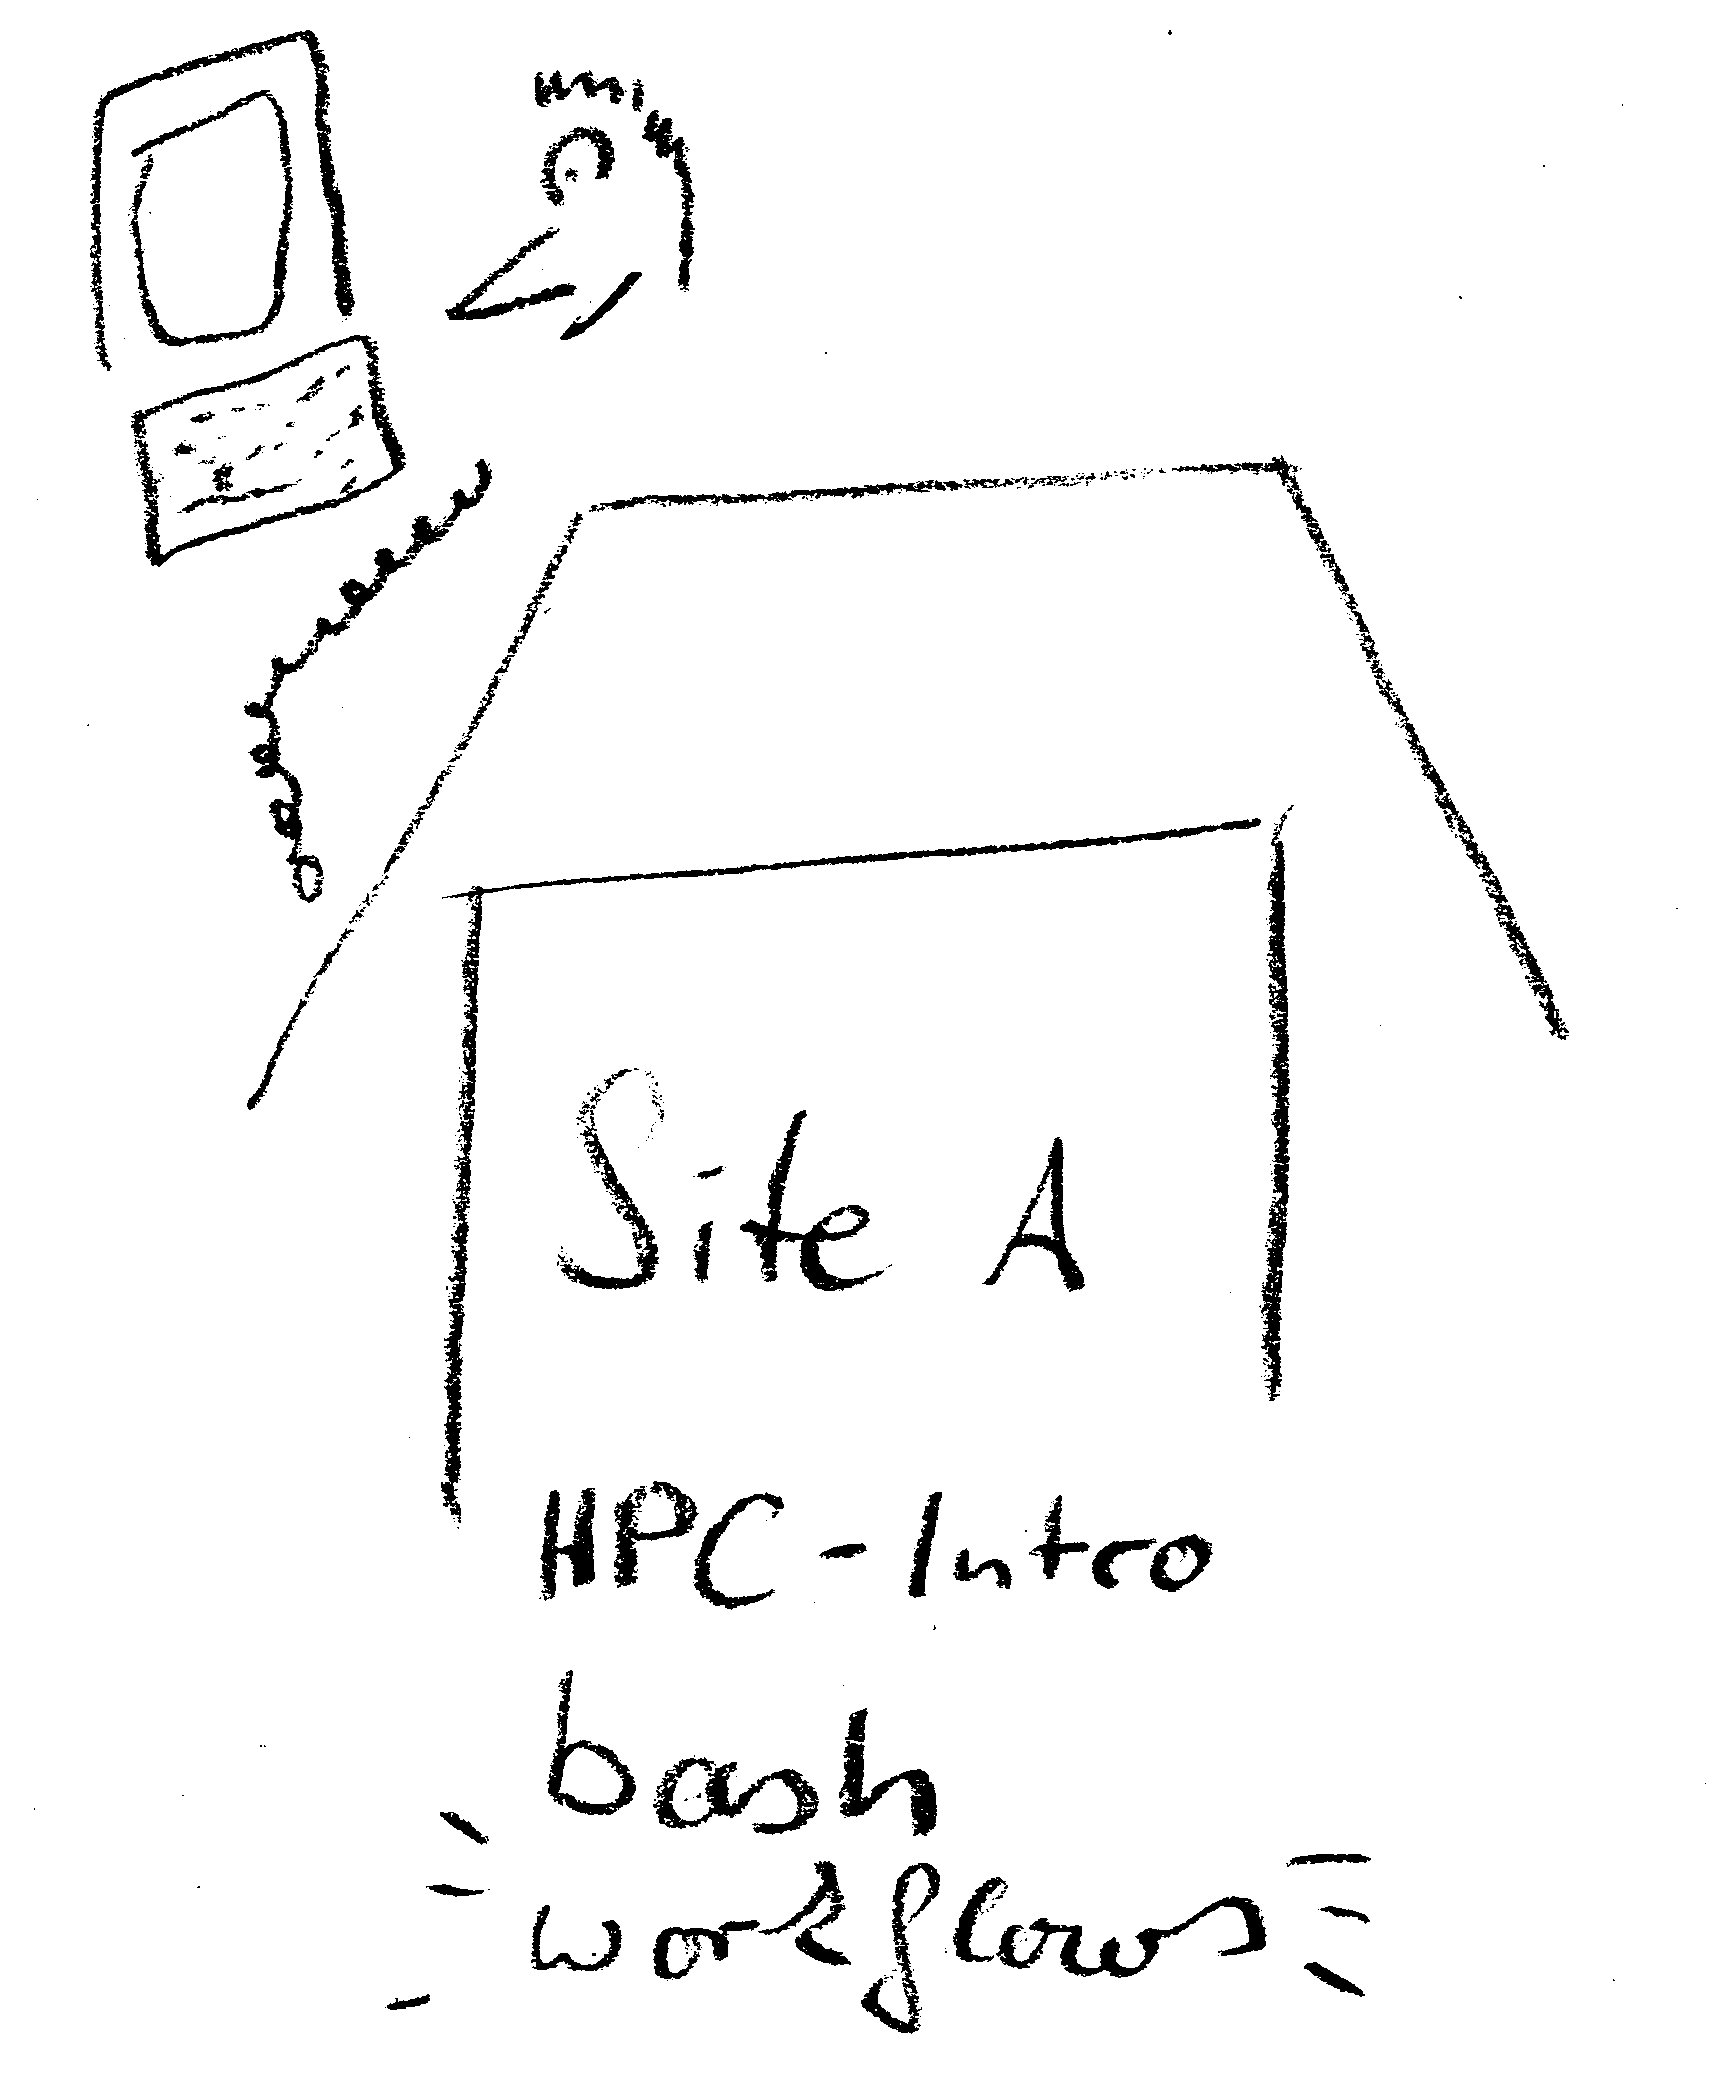
\includegraphics[width=0.7\textwidth]{images/joe}
    \end{column}
    \begin{column}{.5\textwidth}
      \pause
      Most users
      \begin{itemize}[<+->]
        \item \ldots use $3^{rd}$ party applications \ldots
        \item \ldots will need (yet not always visit) an intro course \ldots
        \item \ldots perhaps a scripting course \ldots
        \item \ldots only \emph{really} interested in workflows taylored for their need.
      \end{itemize}
      \pause
      And will never leave their site for other HPC courses!
    \end{column}
  \end{columns}
\end{frame}

%%%%%%%%%%%%%%%%%%%%%%%%%%%%%%%%%%%%%%%%%%%%%%%%%%%%%%%%%%%%%%%%%%%%%%%%%%%%%%%%
\begin{frame}
  \frametitle{HPCCF Adaption as a Plus for Newbies}
  \begin{columns}
   \begin{column}{0.5\textwidth}
    \centering
    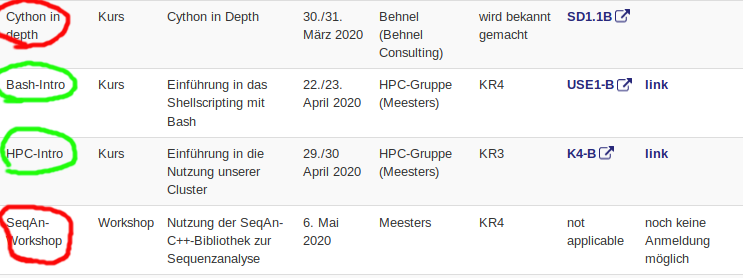
\includegraphics[width=0.8\textwidth]{images/linking_skills_users}\\
    \lhref{https://hpc.uni-mainz.de/kurse-und-workshops/\#bersicht}{Mainz course overview}
   \end{column}
   \begin{column}{0.5\textwidth}
     Assigning HPCCF skill labels to courses is no of cost, yet it will be a plus for ``only-users'':
     \begin{itemize}
      \item will broaden horizons
      \item ``\emph{Maybe} some other course might be interesting, too?''
      \item ``Hm, perhaps more knowledge in this field will be an asset when applying?''
     \end{itemize}
   \end{column}
  \end{columns}
\end{frame}


%%%%%%%%%%%%%%%%%%%%%%%%%%%%%%%%%%%%%%%%%%%%%%%%%%%%%%%%%%%%%%%%%%%%%%%%%%%%%%%%
\begin{frame}
  \frametitle{How Bruce Coder looks on HPC}
  \centering
  {\bcattention \bf \large Exaggeration Warning \bcattention}
  \begin{columns}
    \begin{column}{.6\textwidth}
      \centering
      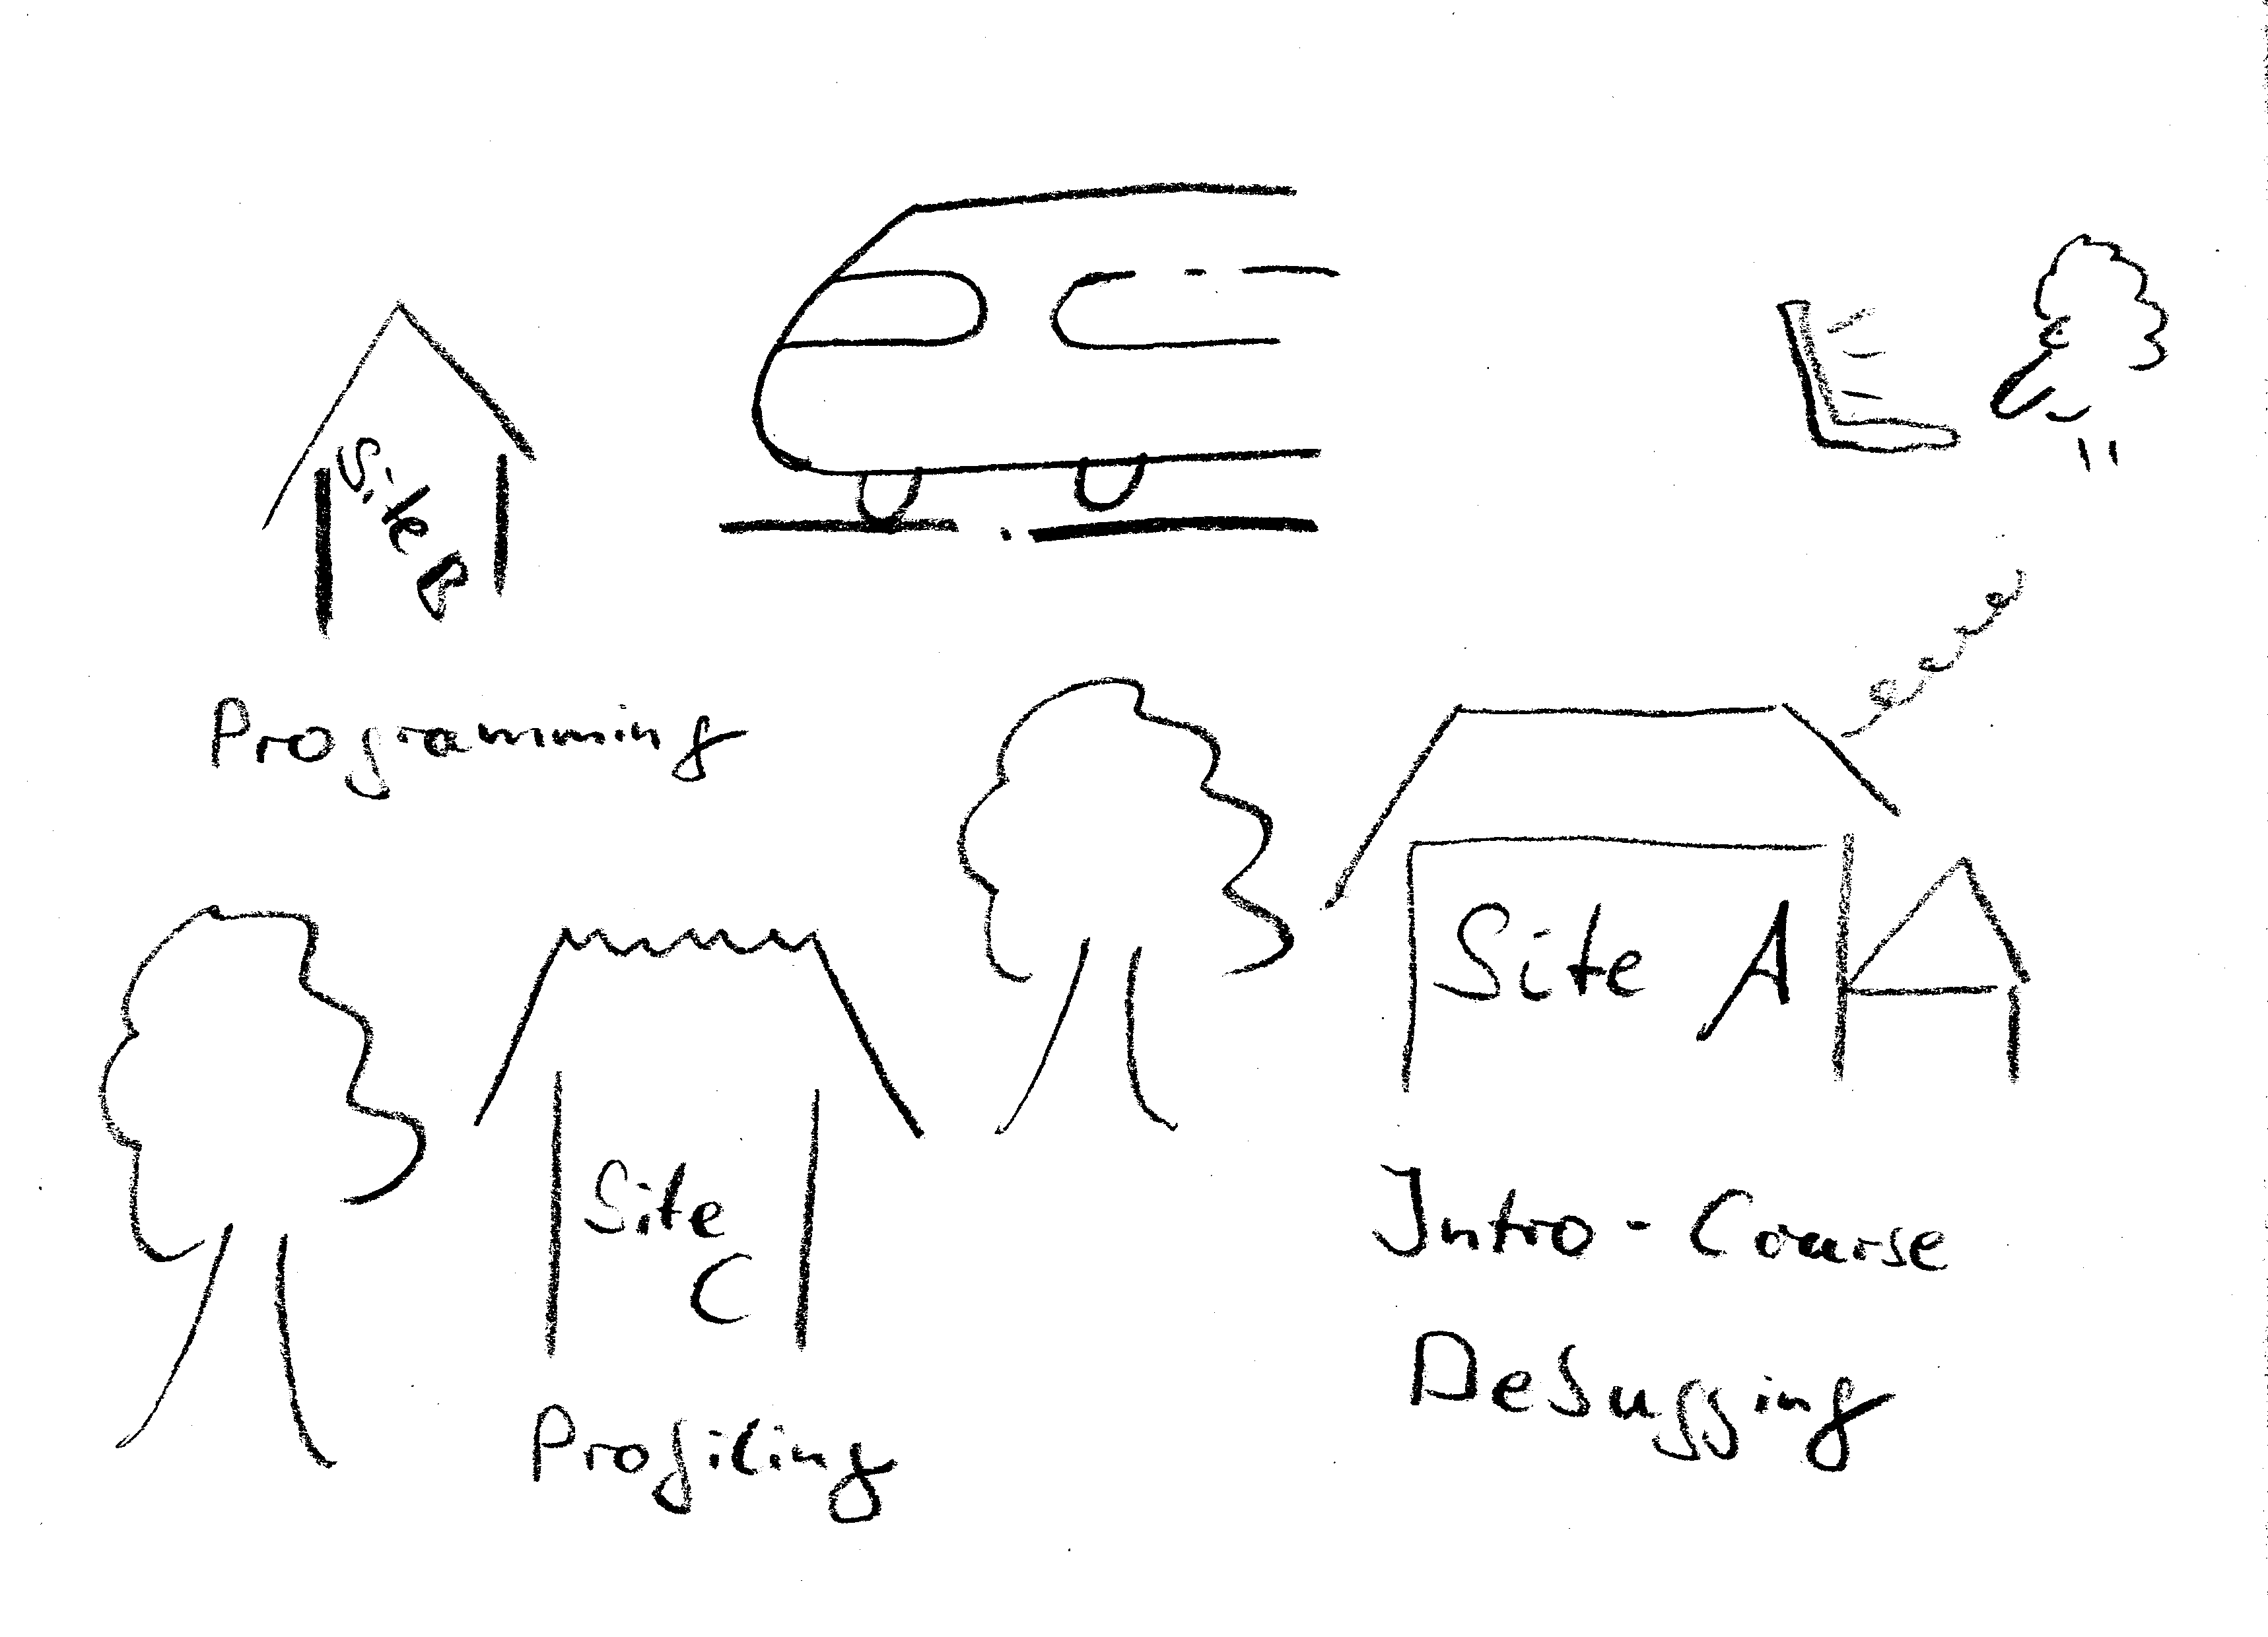
\includegraphics[width=0.8\textwidth]{images/poweruser}
    \end{column}
    \begin{column}{.4\textwidth}
      \pause
      Only power users 
      \begin{itemize}[<+->]
        \item \ldots will select \emph{their} topics \ldots
        \item \ldots will care to travel for computing topics \ldots
        \item \ldots will rarely need intro courses \ldots
      \end{itemize}
    \end{column}
  \end{columns}
\end{frame}

%%%%%%%%%%%%%%%%%%%%%%%%%%%%%%%%%%%%%%%%%%%%%%%%%%%%%%%%%%%%%%%%%%%%%%%%%%%%%%%%
\begin{frame}
  \frametitle{HPCCF a Plus for Power Users}
  \begin{columns}
    \begin{column}{.5\textwidth}
      Advanced Users already use HPC ressources, incl. training. They are aware of
      \begin{itemize}
       \item their local courses
       \item PRACE and other (in-)ternational training resources
      \end{itemize}
    \end{column}
    \begin{column}{.5\textwidth}
      \pause
      Still, they too, will have been newbies at some point \emph{and}
      \begin{itemize}[<+->]
        \item transparency will help them select appropriate courses, too.
        \item ``'Complement my portfolio!''
      \end{itemize}
    \end{column}
  \end{columns}
\end{frame}

\subsection{Certification Process}

\begin{frame}
  \frametitle{Strategy}
  When conceiving a Certification Strategy the different views are in our mind.
  
\end{frame}

\begin{frame}
 \frametitle{Selecting Questions}
 \begin{columns}
    \begin{column}{.5\textwidth}
       \centering
      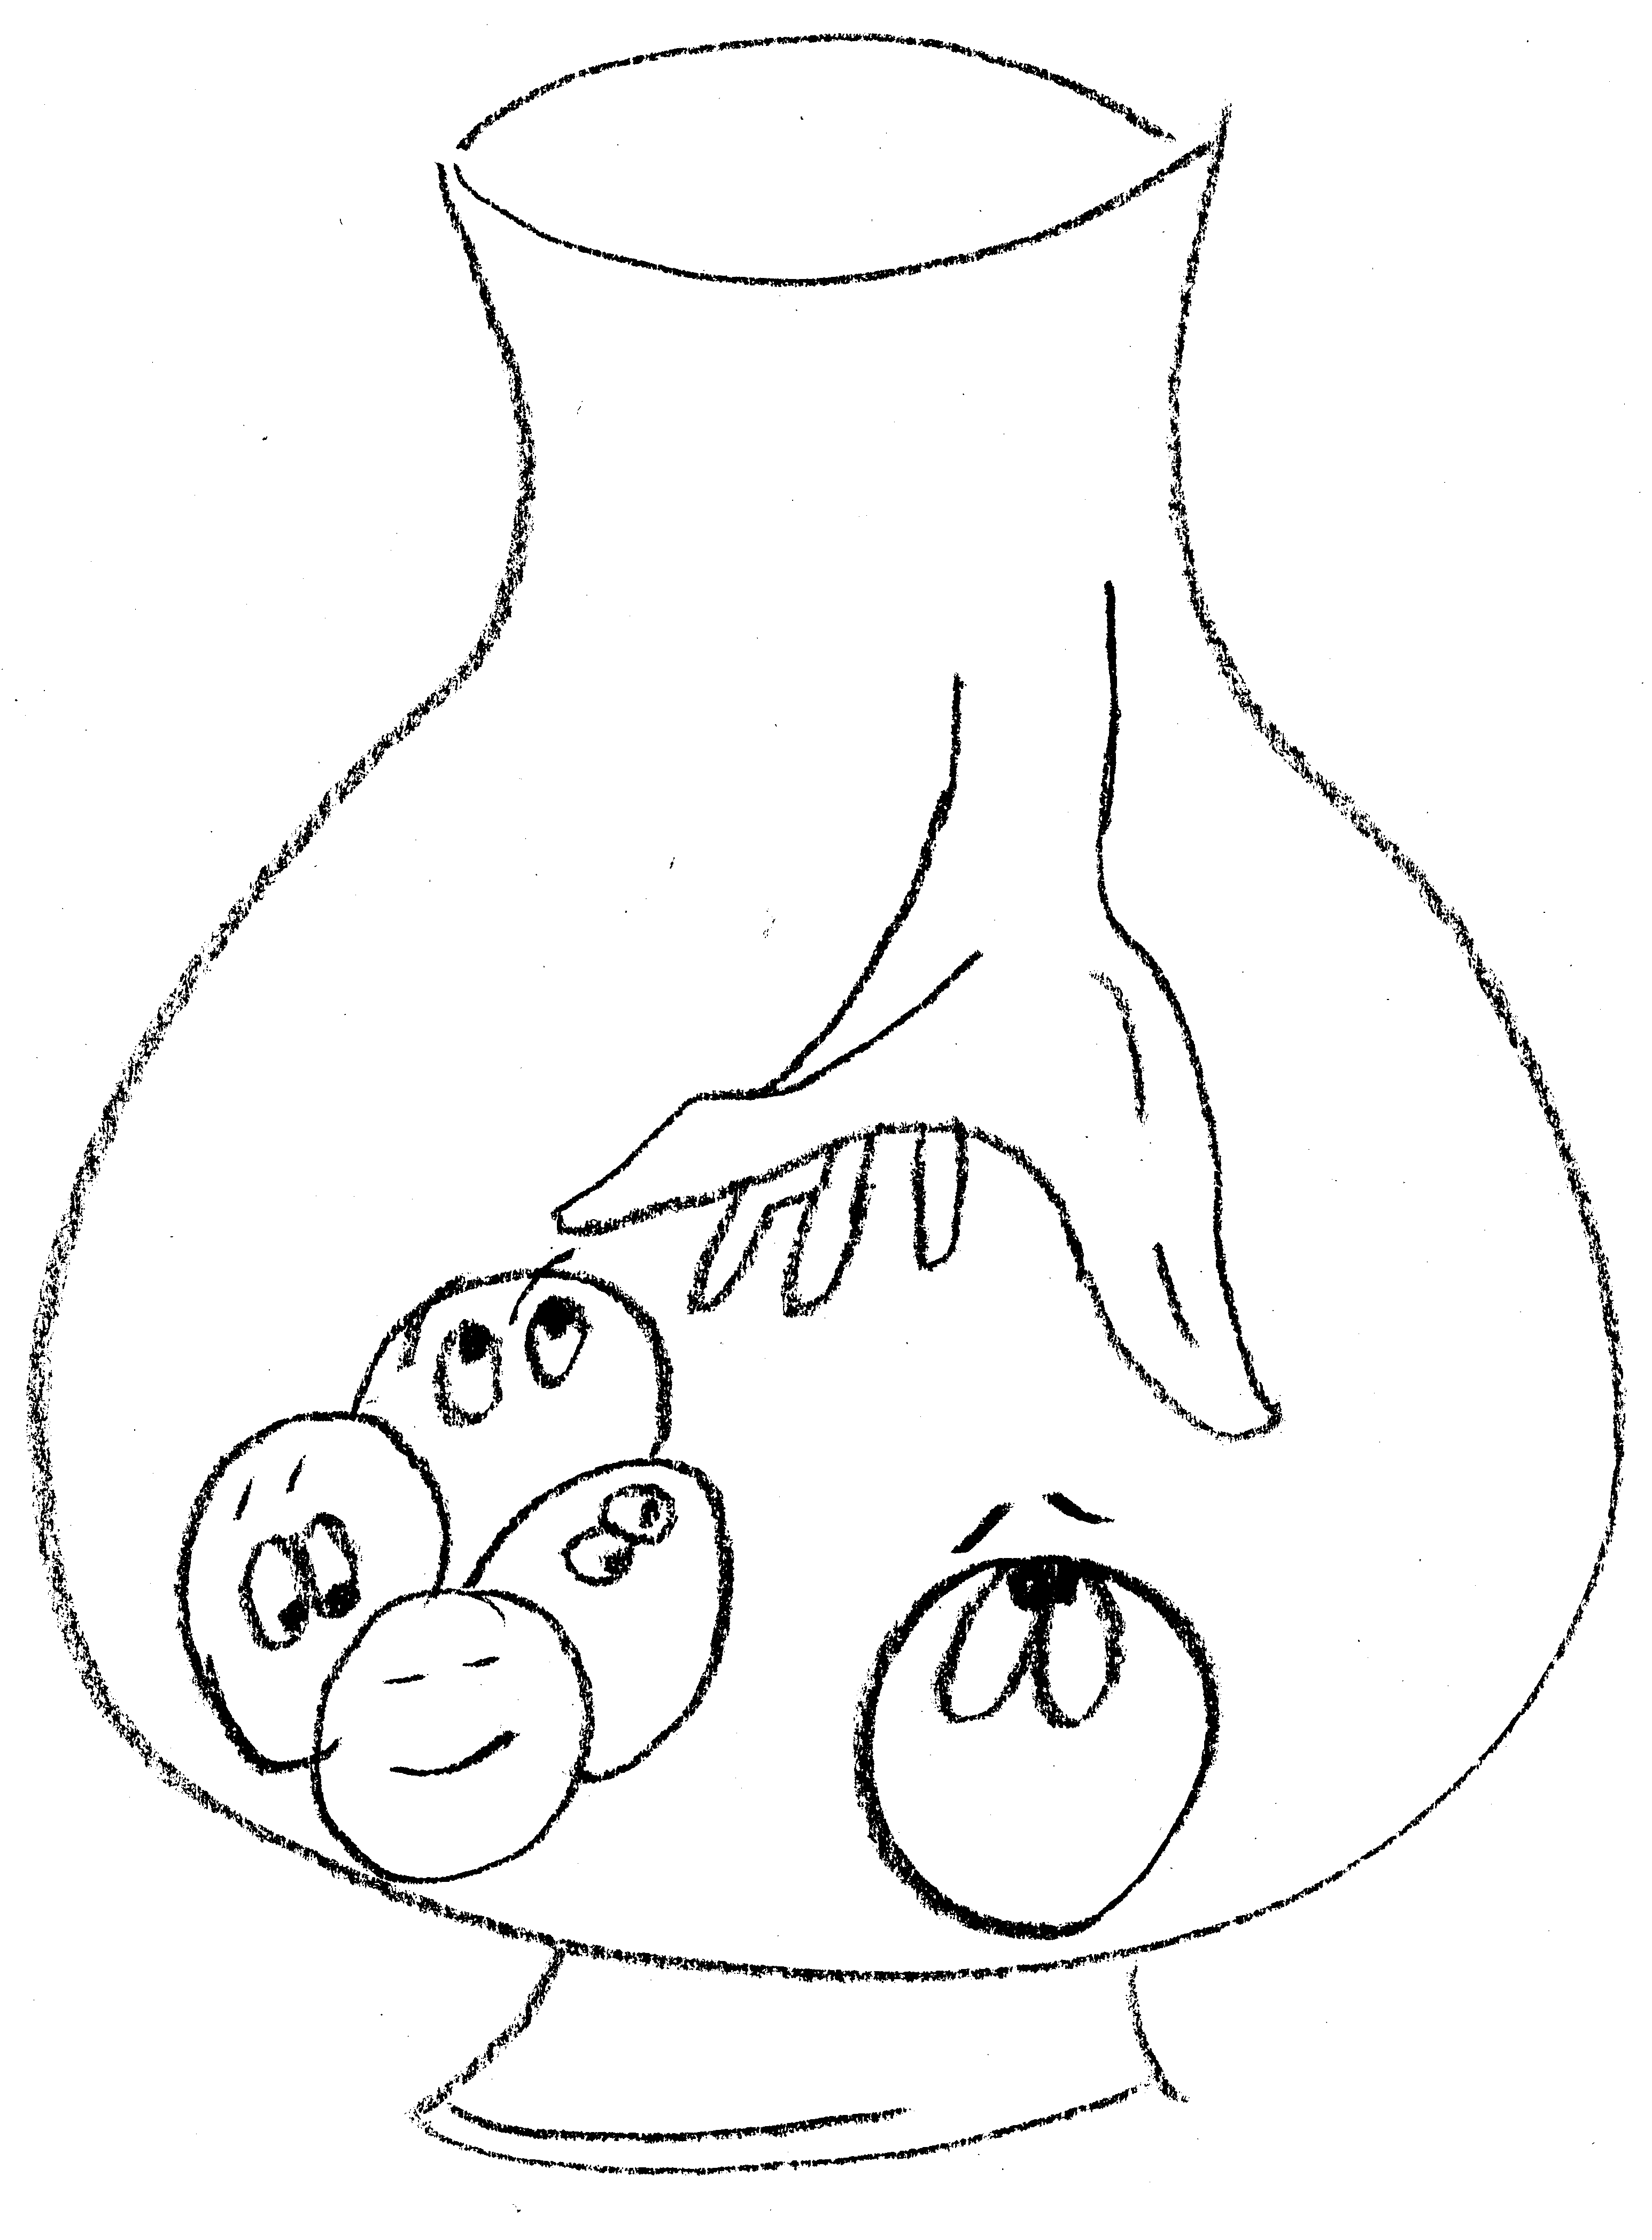
\includegraphics[width=0.6\textwidth]{images/urn}
    \end{column}
    \begin{column}{.5\textwidth}
      Questions are randomly choosen from a pool:
      \begin{itemize}
        \item the pool may itself be a pool of sub-branches of the skill tree
        \item each question will have a pool of right and wrong answers in case of multiple choice questions
      \end{itemize}
      $\curvearrowright$ All examininations will be based on different sets of questions.
    \end{column}
  \end{columns}
\end{frame}

\begin{frame}
  \frametitle{On Cheating}
  \begin{columns}
   \begin{column}{.5\textwidth}
     \begin{enumerate}
      \item By confronting with random questions no perfect preperation can be accomplished.
      \item There is a time-limit per question.
      \item A registration prior to a test session is required.
     \end{enumerate}
    No online system without ID checks and other measures is safe against cheating! Yet, our measures will raise awareness.
   \end{column}
   \begin{column}{.5\textwidth}
       \centering
      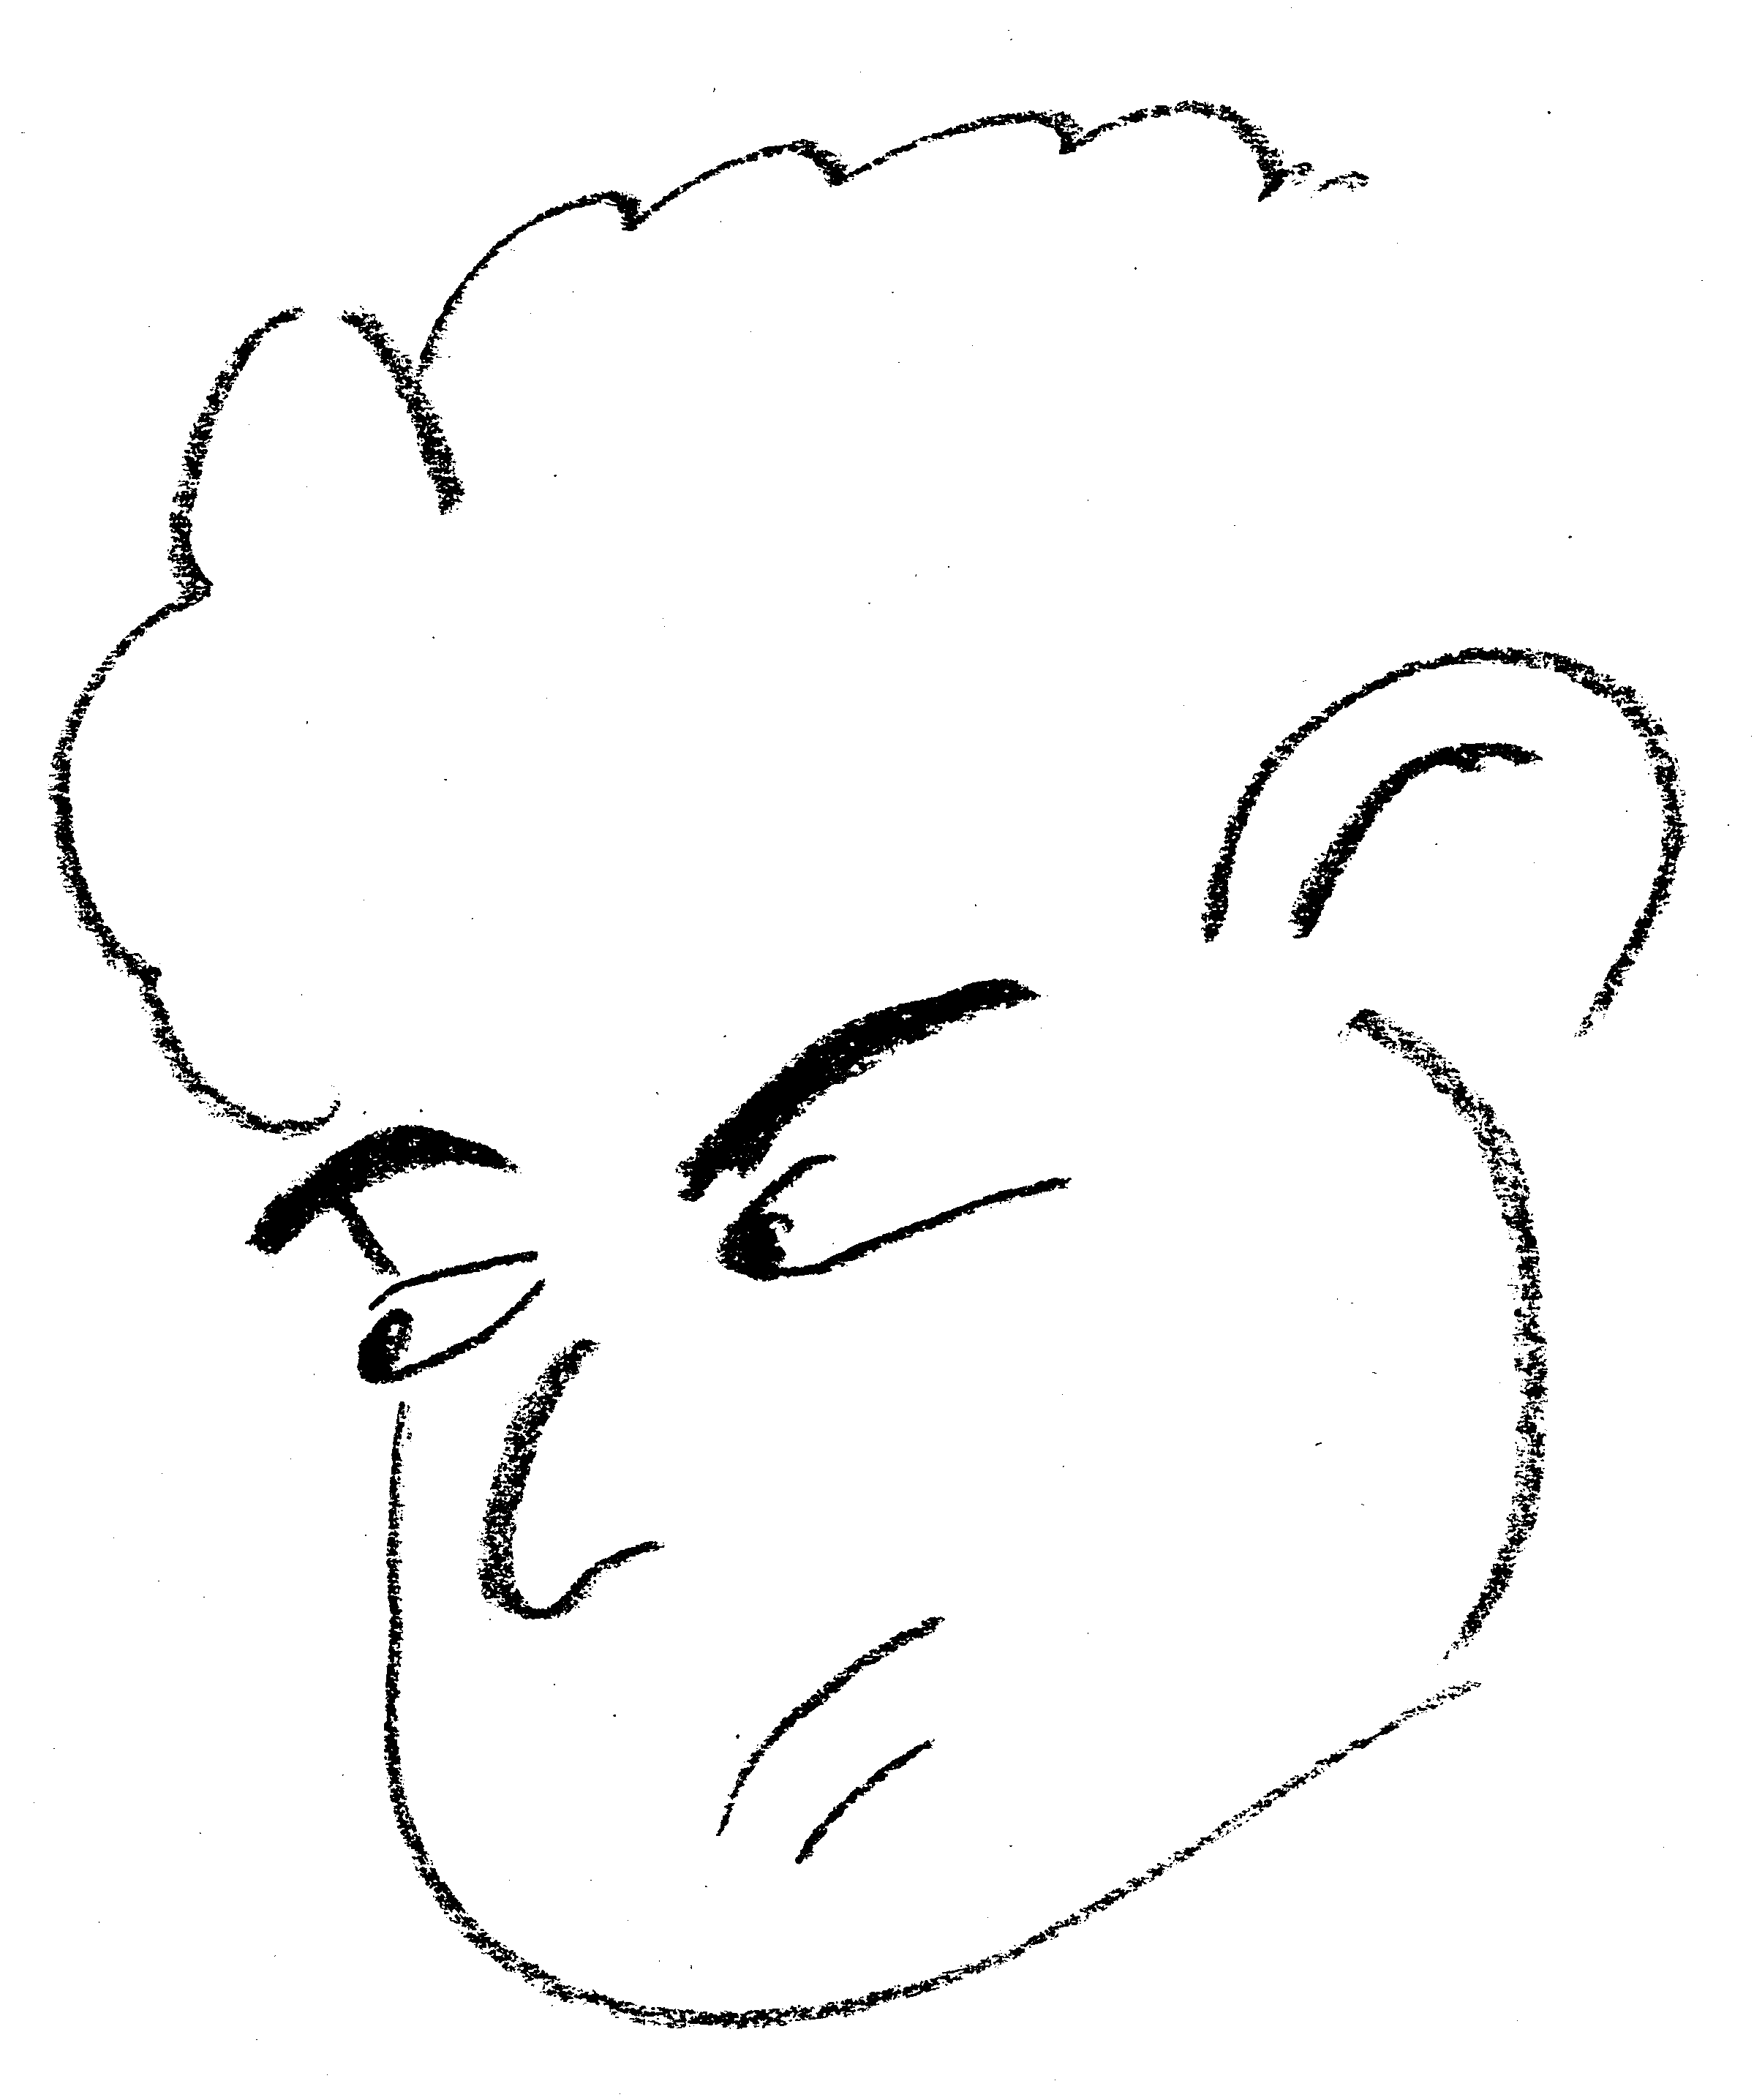
\includegraphics[width=0.6\textwidth]{images/cheating}
    \end{column}
  \end{columns}
\end{frame}

\begin{frame}
 \frametitle{Boosting Acceptance}
 \begin{columns}
   \begin{column}{.5\textwidth}
     Want to hire a scientist? \newline
     We intend to provide a (sub)set of question for prospective employers. This way they will have an idea of the background, if a solicitant waves a HPCCF-certificate.
   \end{column}
   \begin{column}{.5\textwidth}
       \centering
      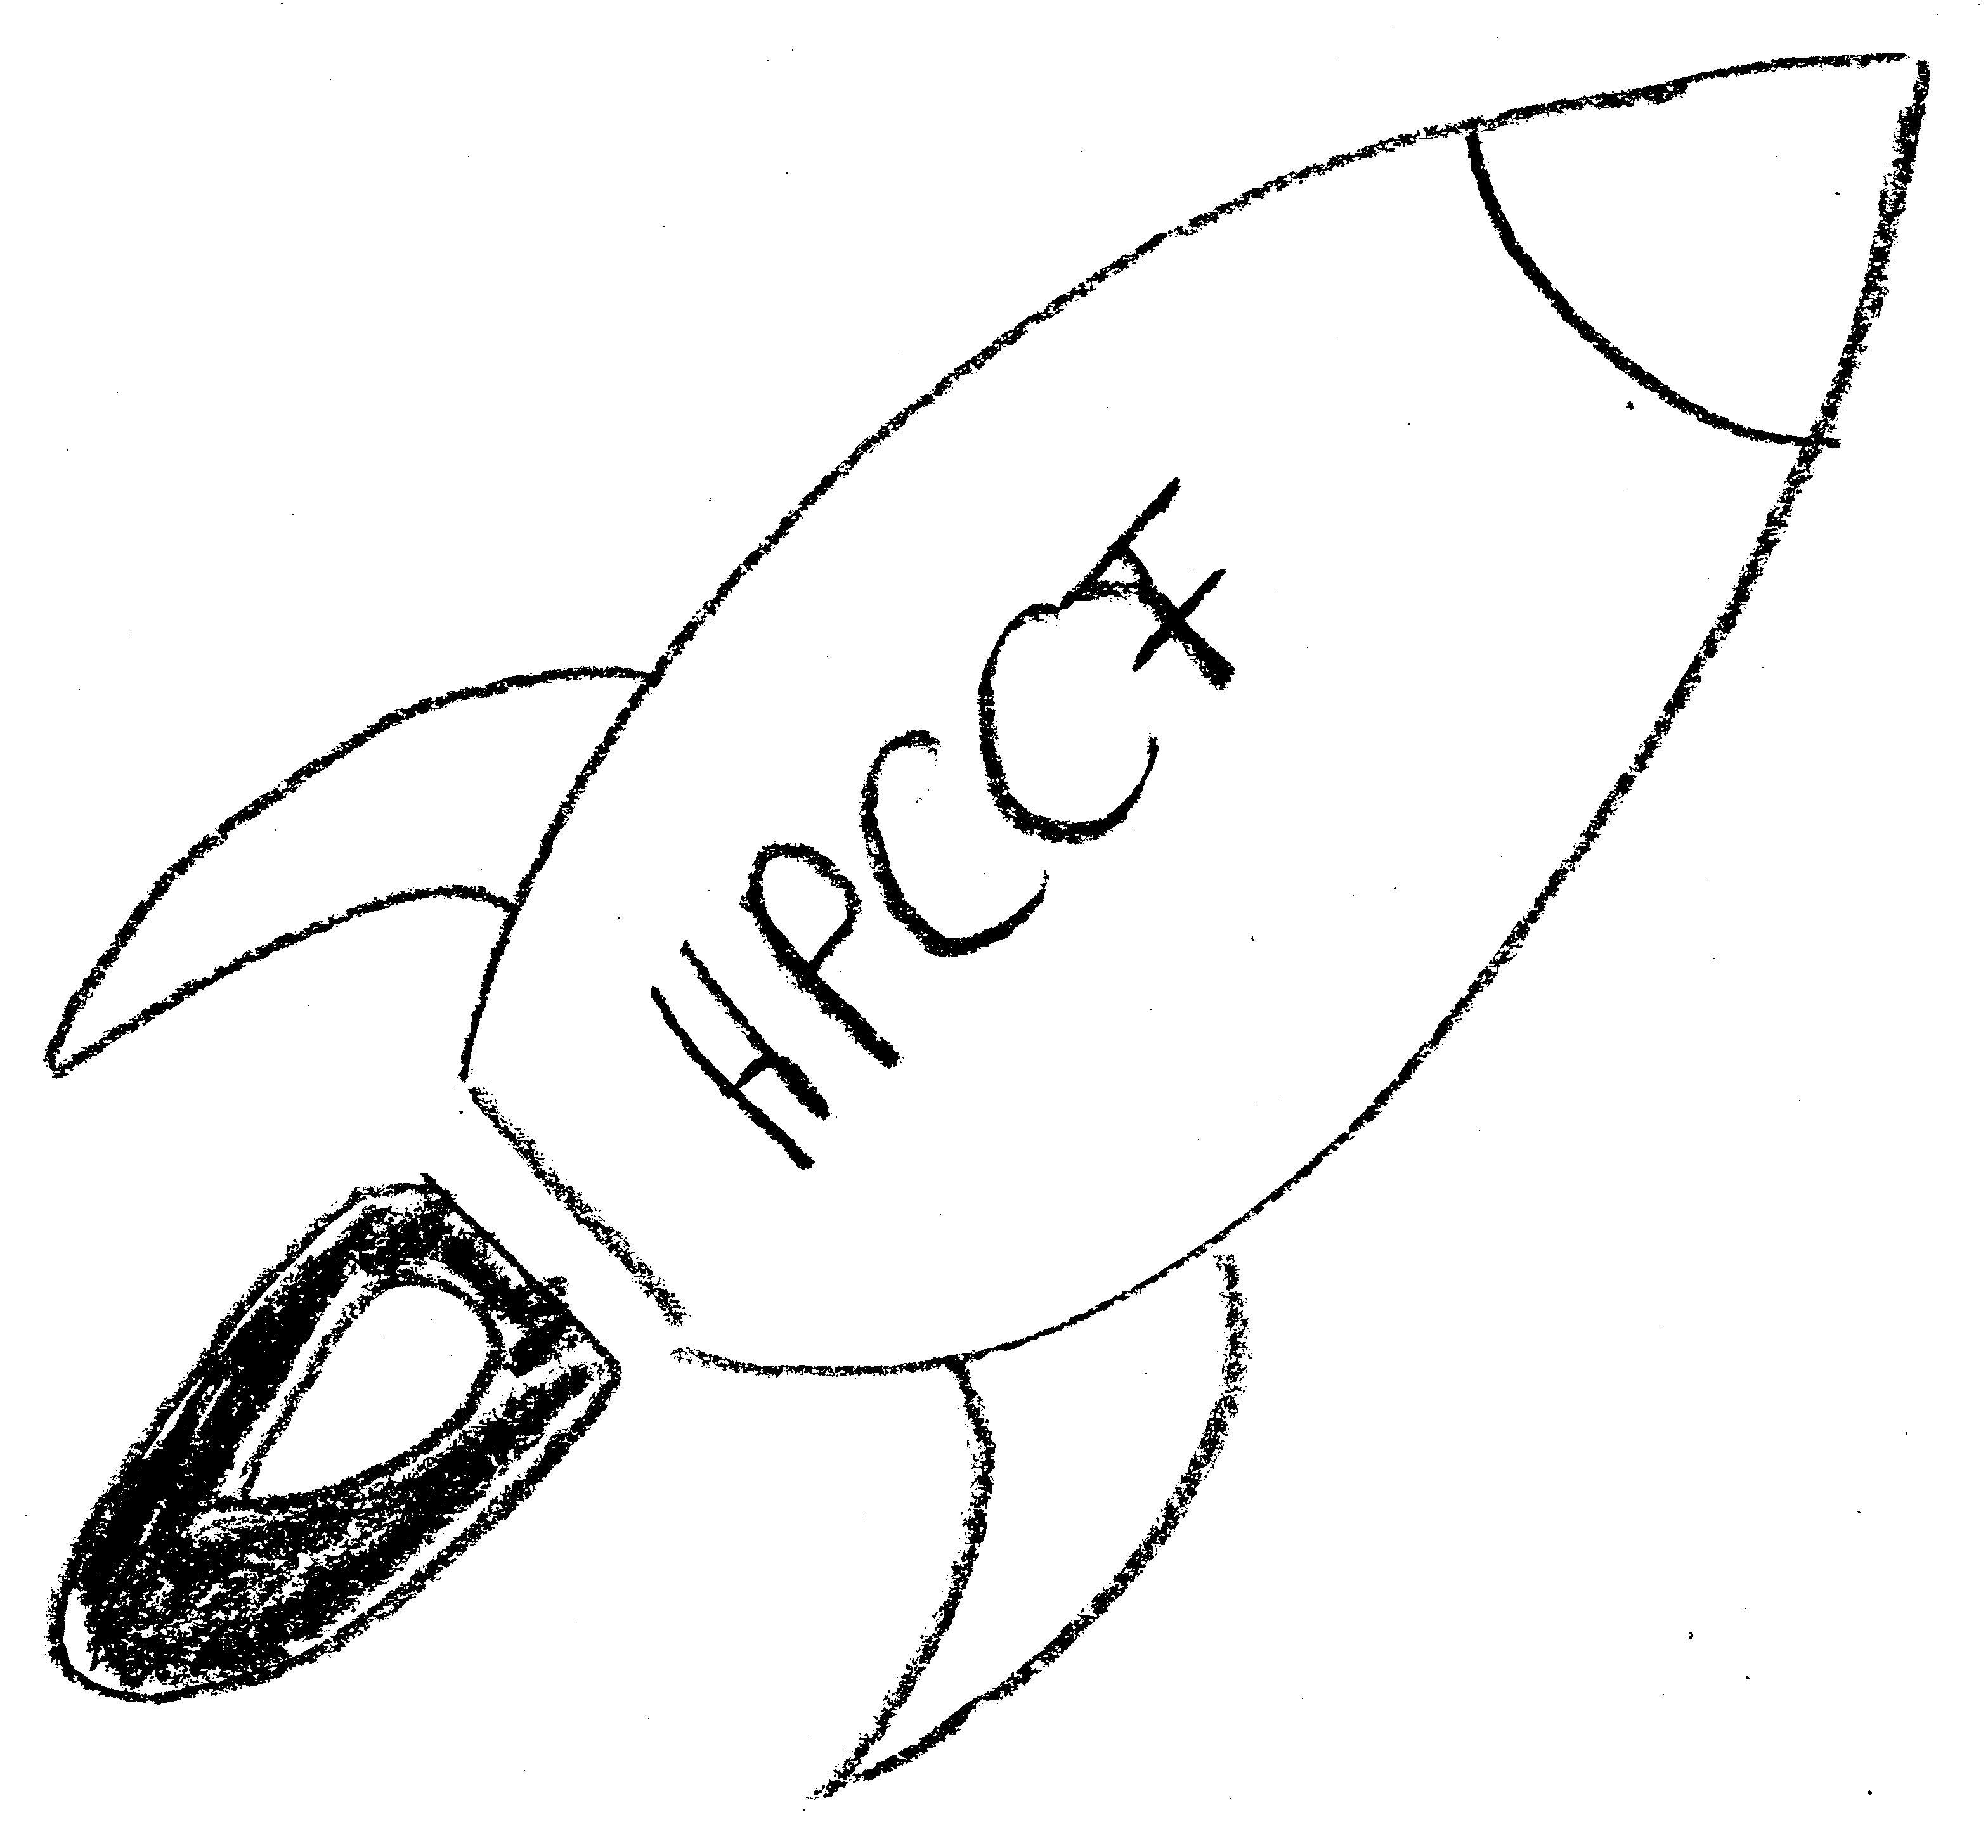
\includegraphics[width=0.6\textwidth]{images/hpccf_boost}
    \end{column}
  \end{columns}
\end{frame}






\section[Designing Questions]{design}

\begin{frame}
  \frametitle{Disclaimer}
  Some examples are inspired by Greg Wilsons book
 \begin{center}
  \sf{Teaching Tech Together} (CRC Press, 2020)
 \end{center}
 Some ideas are based on own experience, some on other sources.
\end{frame}

\subsection{Question Types}

\begin{frame}
  \frametitle{Purposes \ldots}
  Before diving into Question Design, note:
  \begin{itemize}
    \item a question can be asked with a certain aim
    \item different courses ask for different knowledge / skills
    \item $\curvearrowright$ questions need to be designed and choosen with care
  \end{itemize}
\end{frame}

% overview
% background selection

\subsection{Multiple Choice Questions}

\begin{frame}
 \frametitle{Multiple Choice -- When?}

 Multiple Choice Questions (MCQs) are popular when designing e-learning tests \ldots\vspace{-1em}
 \pause
 \newline
 \only<2->{\question{When are they most suitable?}}
 \pause
 Suppose you are teaching children and you give them this MCQ:
 \exercise[Testing Conceptions]{
  What is 37 + 15?
  \begin{enumerate}[a)]
   \item 52  {\color{pdarkgrey}correct}
   \item 42  {\color{pdarkgrey}child did not understand ``carrying''}
   \item 412 {\color{pdarkgrey}child treated every column seperately}
   \item 43  {\color{pdarkgrey}knows she has to carry 1, but to wrong column}
  \end{enumerate}
 }
\end{frame}


\begin{frame}
 \frametitle{Multiple Choice -- When? (continued)}
 
 The Young-Child question rephrased for newbies to the SLURM batch system:
 \vspace{-1em}
 \exercise[Testing Conceptions about SLURM]{
   Think of a cluster with 20 core nodes. If a job is submitted with the following parameterisation, how many nodes are reserved?\newline
   \texttt{\#SBATCH -n 20}\newline
   \texttt{\#SBATCH -c 2}
   \begin{enumerate}[a)]
    \item 2 {\color{pdarkgrey}correct}
    \item 4 {\color{pdarkgrey}user did correctly multiply, but is not aware of the 20 cores}
    \item 1 {\color{pdarkgrey}user did not multiply by \texttt{-c 2}}
    \item unkown without \texttt{N}-flag {\color{pdarkgrey}user did not understand the concept}
   \end{enumerate}
  }
\end{frame}

\begin{frame}
  \frametitle{What is in the Arsenal?}
  \begin{columns}
   \begin{column}{.5\textwidth}
    MCQs aren't everything:
     \begin{enumerate}
      \item Freetext (if short and explicit)
      \item Filling in blanks (for code; to be implemented)
      \item Parson Problem (can by done as MCQ; in a minute)
      \item Tracing (can by done as MCQ; in a minute)
     \end{enumerate}
   \end{column}
   \begin{column}{.5\textwidth}
       \centering
      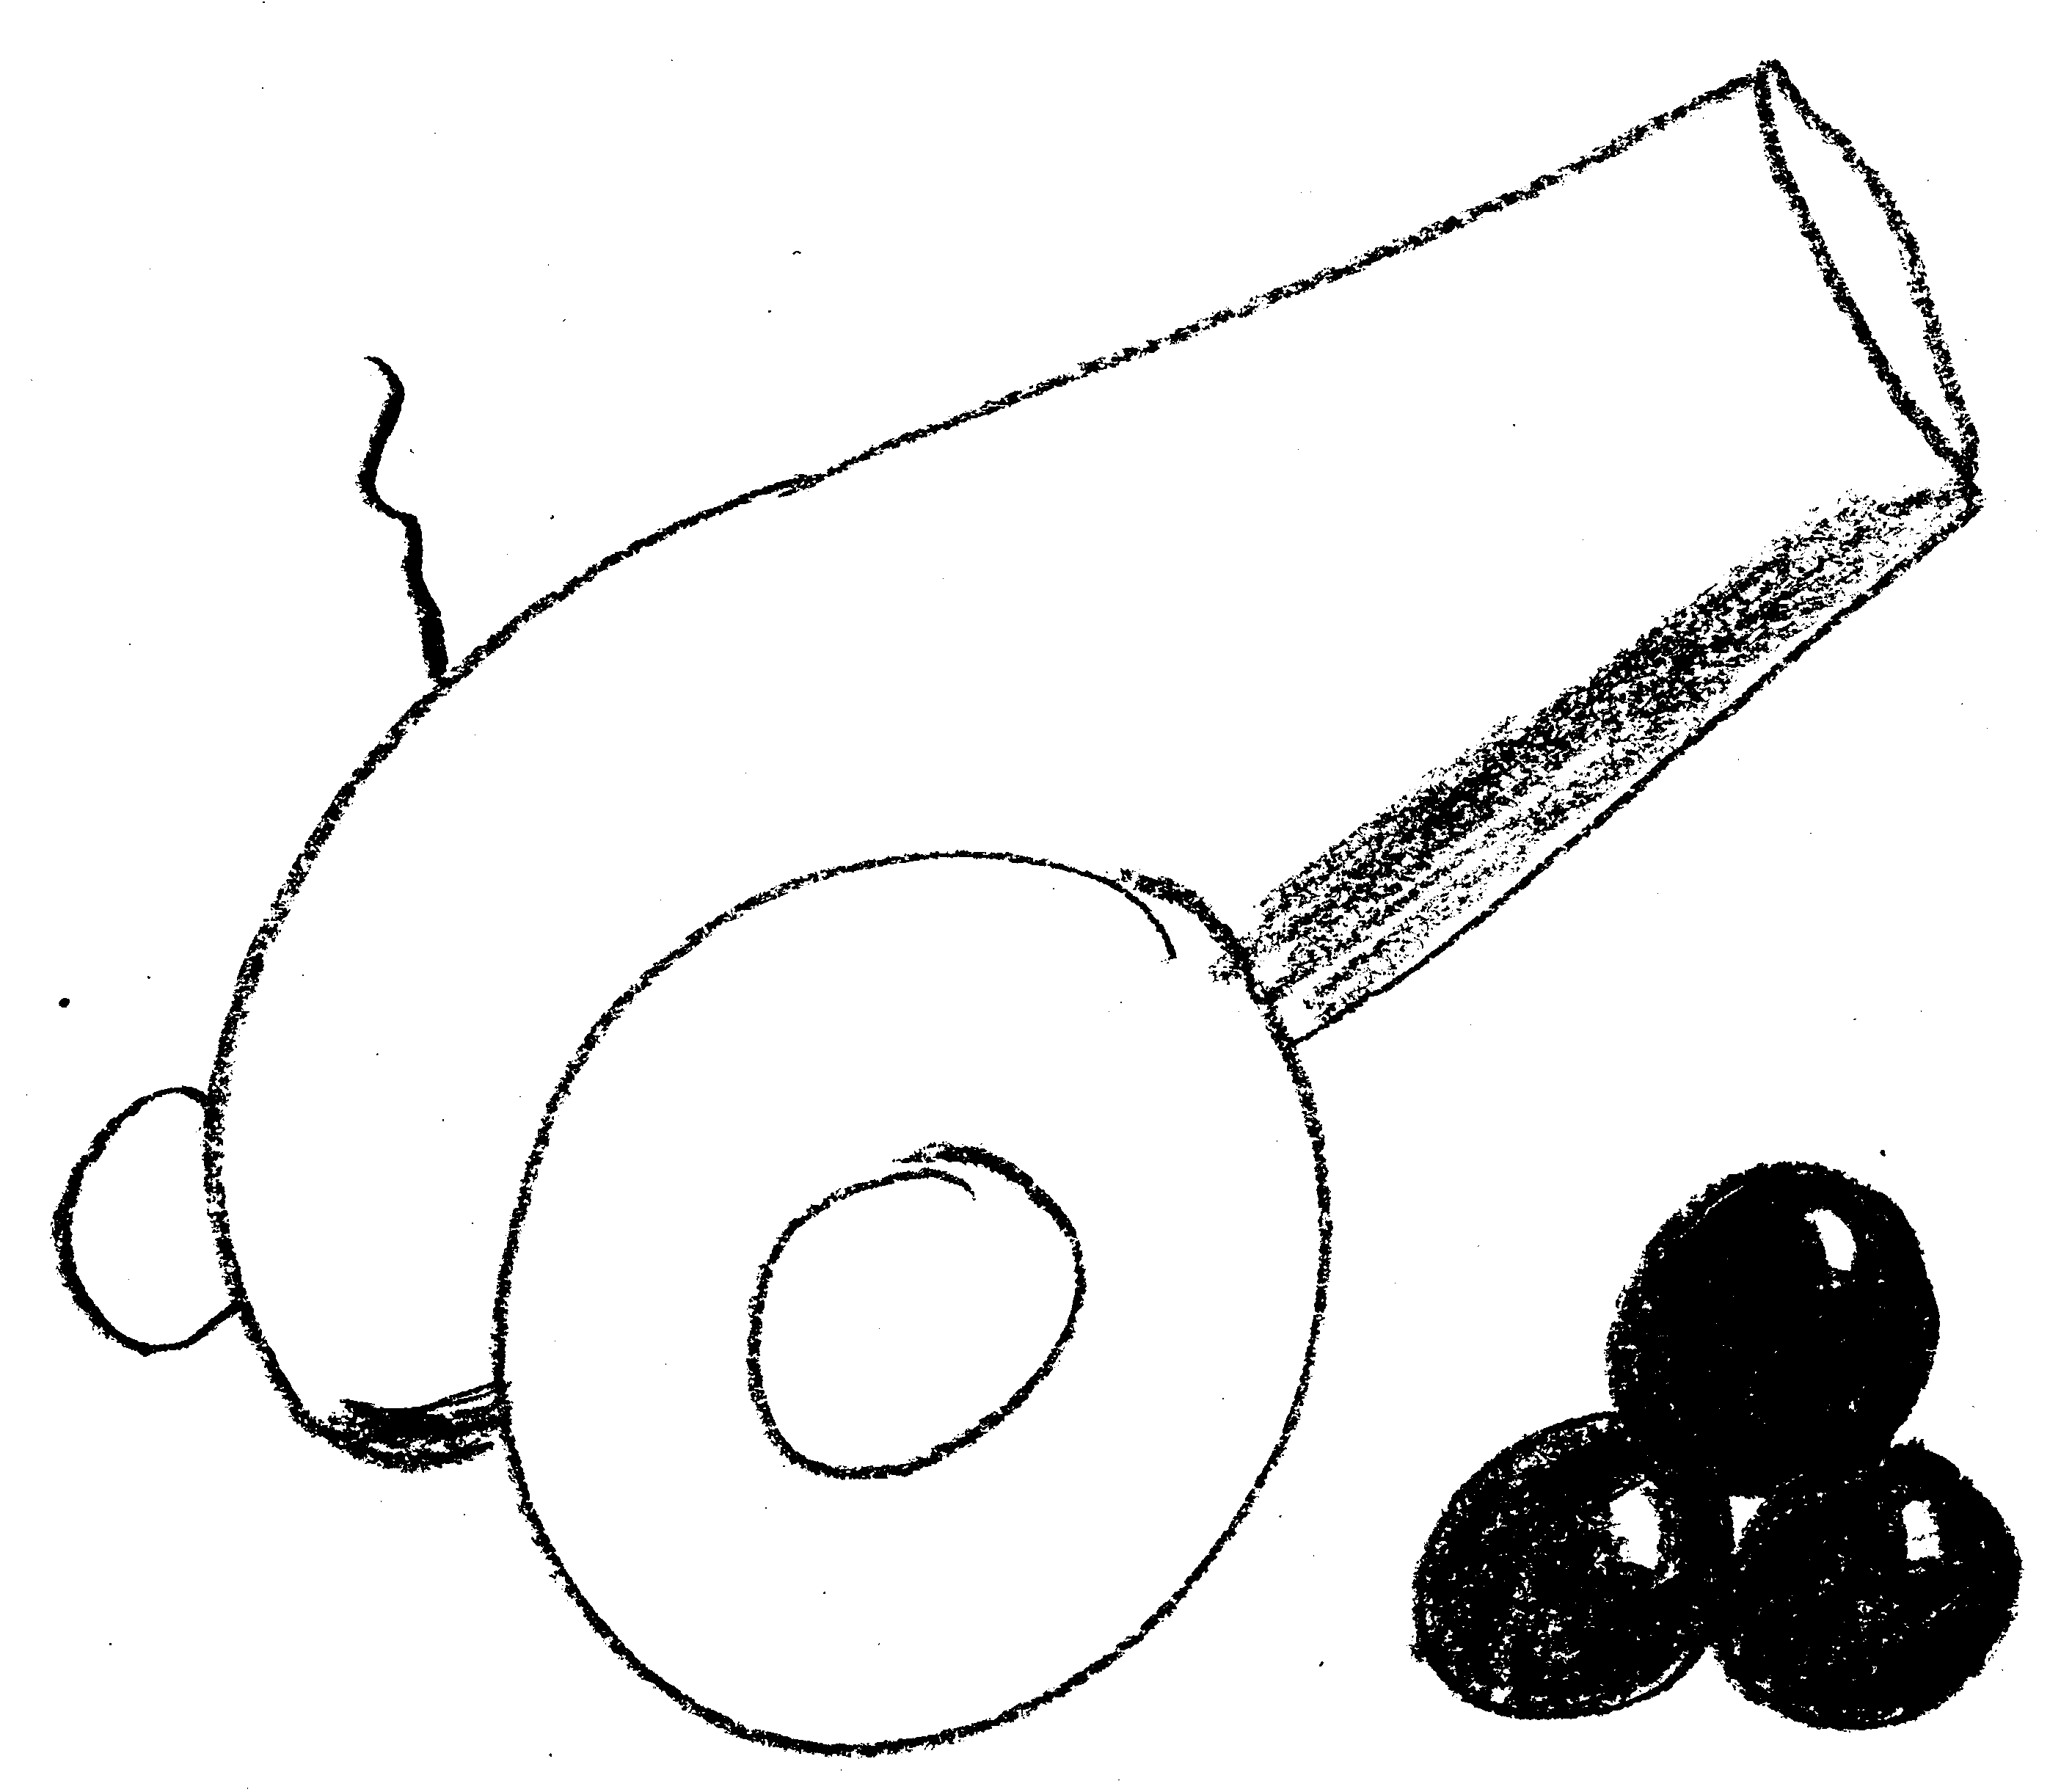
\includegraphics[width=0.6\textwidth]{images/arsenal}
    \end{column}
  \end{columns}
\end{frame}

\begin{frame}
  \frametitle{Freetext}
  Freetext question need to be \emph{very} much restricted to simple words or characters. For example:
  \exercise[Changing Permissions]{
           If a script file 'foo.sh' has the permissions '-rw-r--r--', 
           how do make it executable for your group for sharing the script?
           }
  Here, only two possible answers are allowed, in octal or explicit mode.
  \pause
  \hint[Most Suitable]{This kind is of question is most suitable to test actual knowledge. As we can expect only few students to memorize all nifty details, it primarly tests for gained experience and is to be used with great care (not to frequent).}
\end{frame}

\begin{frame}
  \frametitle{Fill in Blanks}
  Filling Blanks is a (technical) variation on Freetext. It is more specific and the \emph{blank screen of horror} problem, whilst testing vocabulary. An example:
  \exercise[Bash Operators]{
            Which operator has to be filled in the place of '\_' to print the statement in line 3?\newline
            {\small \bf 1:} \texttt{number=4}\newline
            {\small \bf 2:} \texttt{if [ \$((number {\color{red}\bf\_} 2 )) -eq 0 ]; then}\newline
            {\small \bf 3:} \texttt{~~~~echo "\$number is even"}\newline
            {\small \bf 4:} \texttt{fi}
            }
  \hint{The answer is a single character.}
\end{frame}

\begin{frame}
  \frametitle{Parsons Problems}
  Parsons Problems, too, avoid the \emph{blank screen of horror} problem and also the vocabulary testing. Instead they allow the examinee to concentrate on the control flow. 
  \vspace{-.5em}
  \begin{columns}
    \begin{column}{.7\textwidth}
      \exercise[Bash Loop \& Math]{
                Rearrange these lines to sum the values.\newline
                {\small \bf 1:} \texttt{done}\newline
                {\small \bf 2:} \texttt{values=(1 2 3 4)}\newline
                {\small \bf 3:} \texttt{for v in \${values[@]}; do}\newline
                {\small \bf 4:} \texttt{total=\$((total + v))}\newline
                }
    \end{column}
    \begin{column}{.3\textwidth}
      Real tasks can be longer and intricated - allowing test of control flow understanding.
    \end{column}
  \end{columns}
  \vspace{-.5em}
  \hint[Note]{The answer can be a free text, e.\,g.: ``2 3 4 1'', which is easy to parse and check.}
\end{frame}

\begin{frame}[t]
  \frametitle{What else?}
  We could go on \ldots
  \vspace{1em}
  \begin{columns}
    \begin{column}{.7\textwidth}
      \centering
      \begin{tabular}{p{.25\textwidth}p{.55\textwidth}}
         Exercise Type & Technical Implementation\\\hline
         Tracing Code Execution & \only<2->{Freetext or MCQ}\\
         Labelling Diagrams & \only<3->{MCQ}\\
         Fixing Code & \only<4->{Freetext}\\
         etc & \only<5->{Variety of types with minimal technical effort.}
      \end{tabular}
    \end{column}
    \begin{column}{.3\textwidth}
      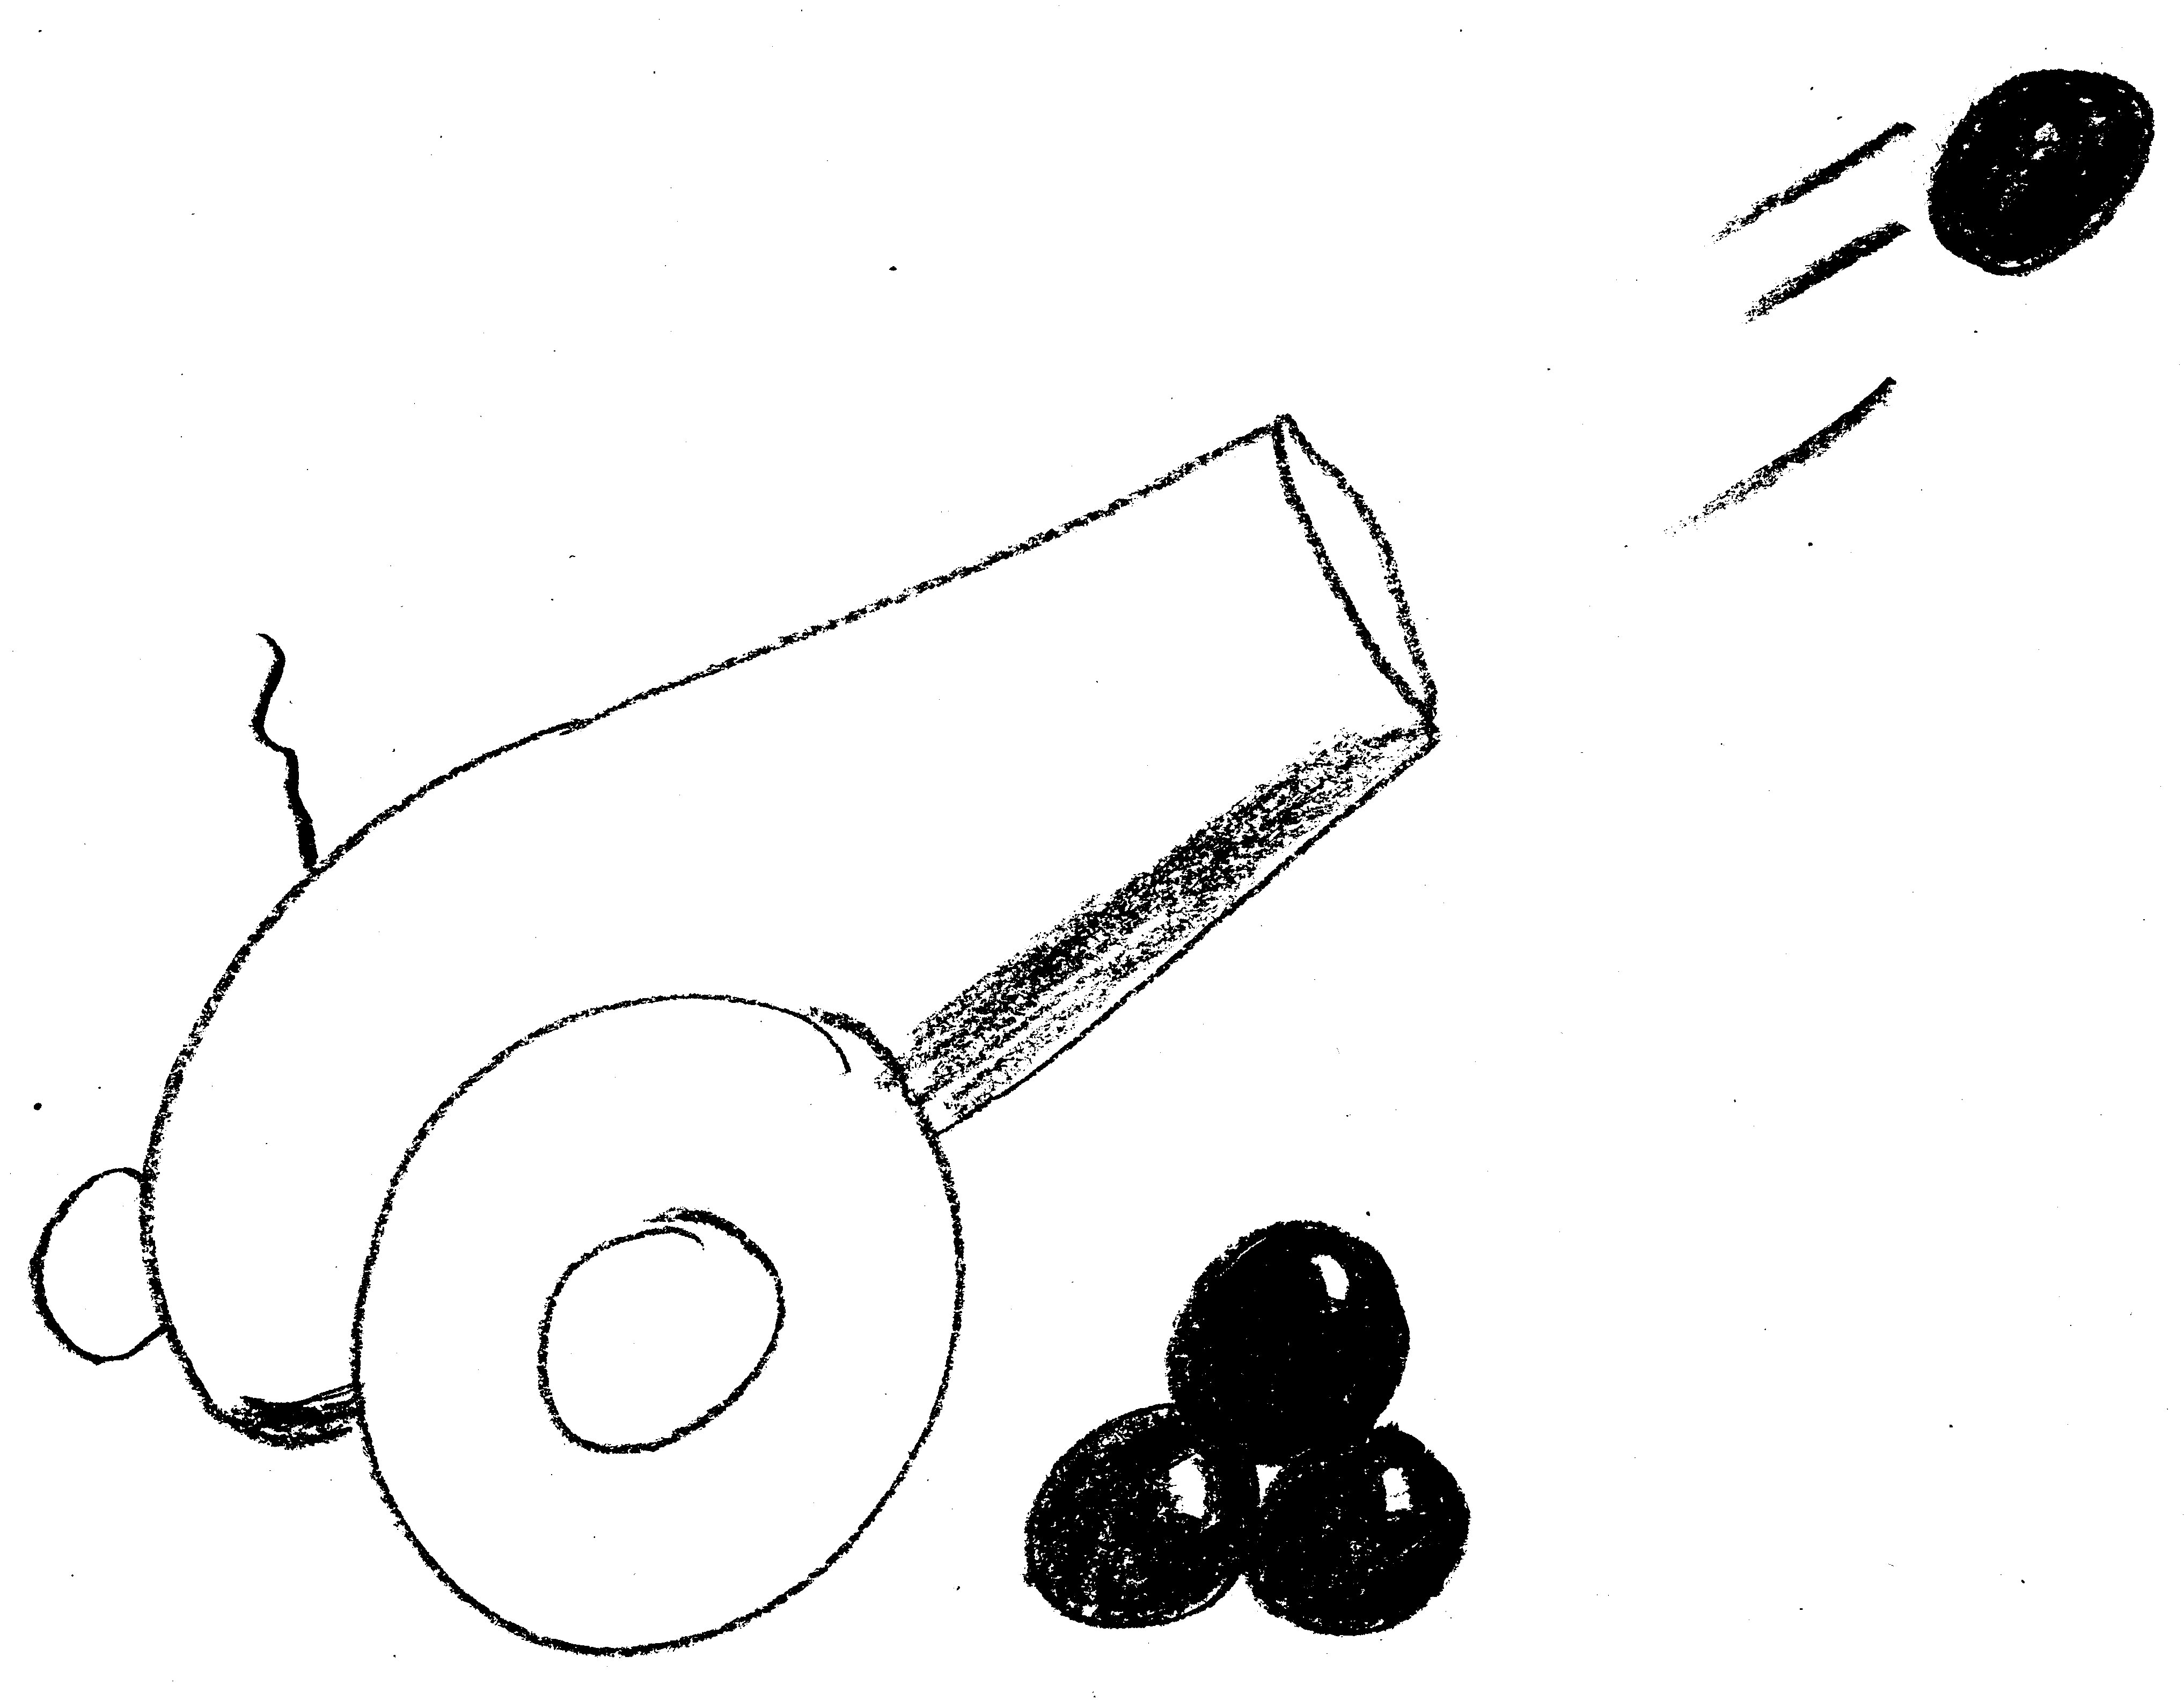
\includegraphics[width=0.6\textwidth]{images/arsenal2}
    \end{column}
   \end{columns}
\end{frame}



\section[Contributing to the Question Pool]{Contributing}

\begin{frame}
  \frametitle{Contributions via the HPCCF-Wiki}
  \centering
  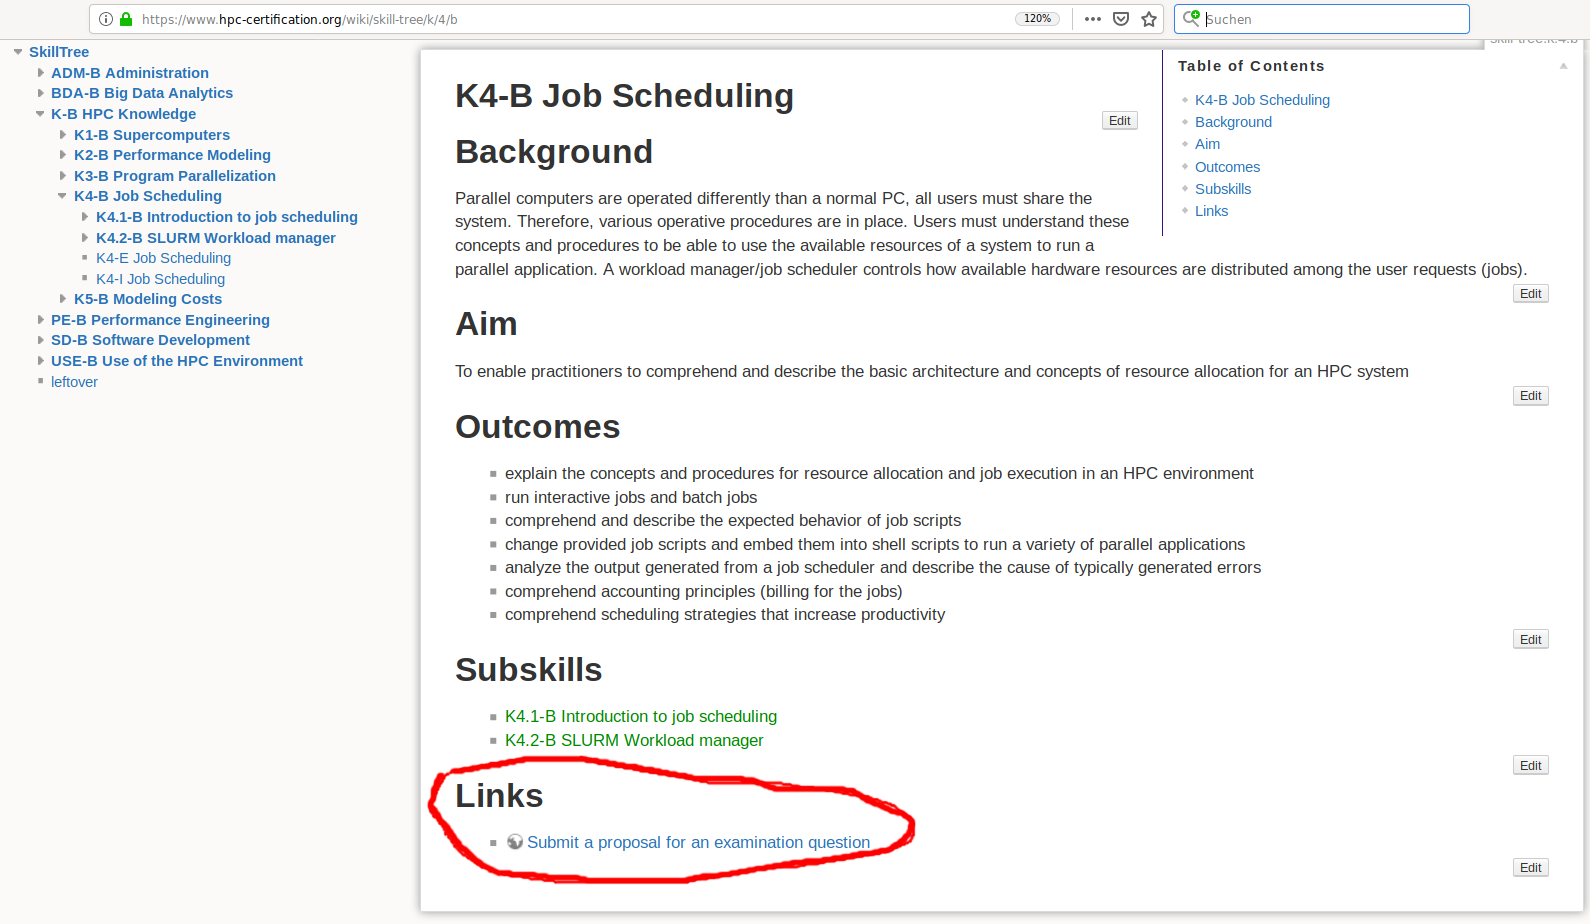
\includegraphics[width=0.8\textwidth]{images/contribution}
\end{frame}


\begin{frame}
  \frametitle{Contributions via the HPCCF-Wiki II}
  Each \lhref{https://www.hpc-certification.org/wiki}{HPCCF wiki} page contains a link. It leads to a little form asking for:
  \begin{itemize}
   \item contact mail
   \item to select a learning objective from a pre-formatted list
   \item to supply the question you thought of
   \item and (in case of a multiple choice question) the possible answers.
  \end{itemize}
  \pause
  \task[Evaluation Process]{Now, HPCCF-member evaluate the submitted question. If approved, it will be formatted and merged into the pool of questions for the choosen topic / skillset.}
\end{frame}



\begin{frame}
 \centering
 \begin{columns}
   \begin{column}{0.8\textwidth}
     \centering
     \Large
     Thank You for Your Attention!
   \end{column}
   \begin{column}{0.2\textwidth}
     
      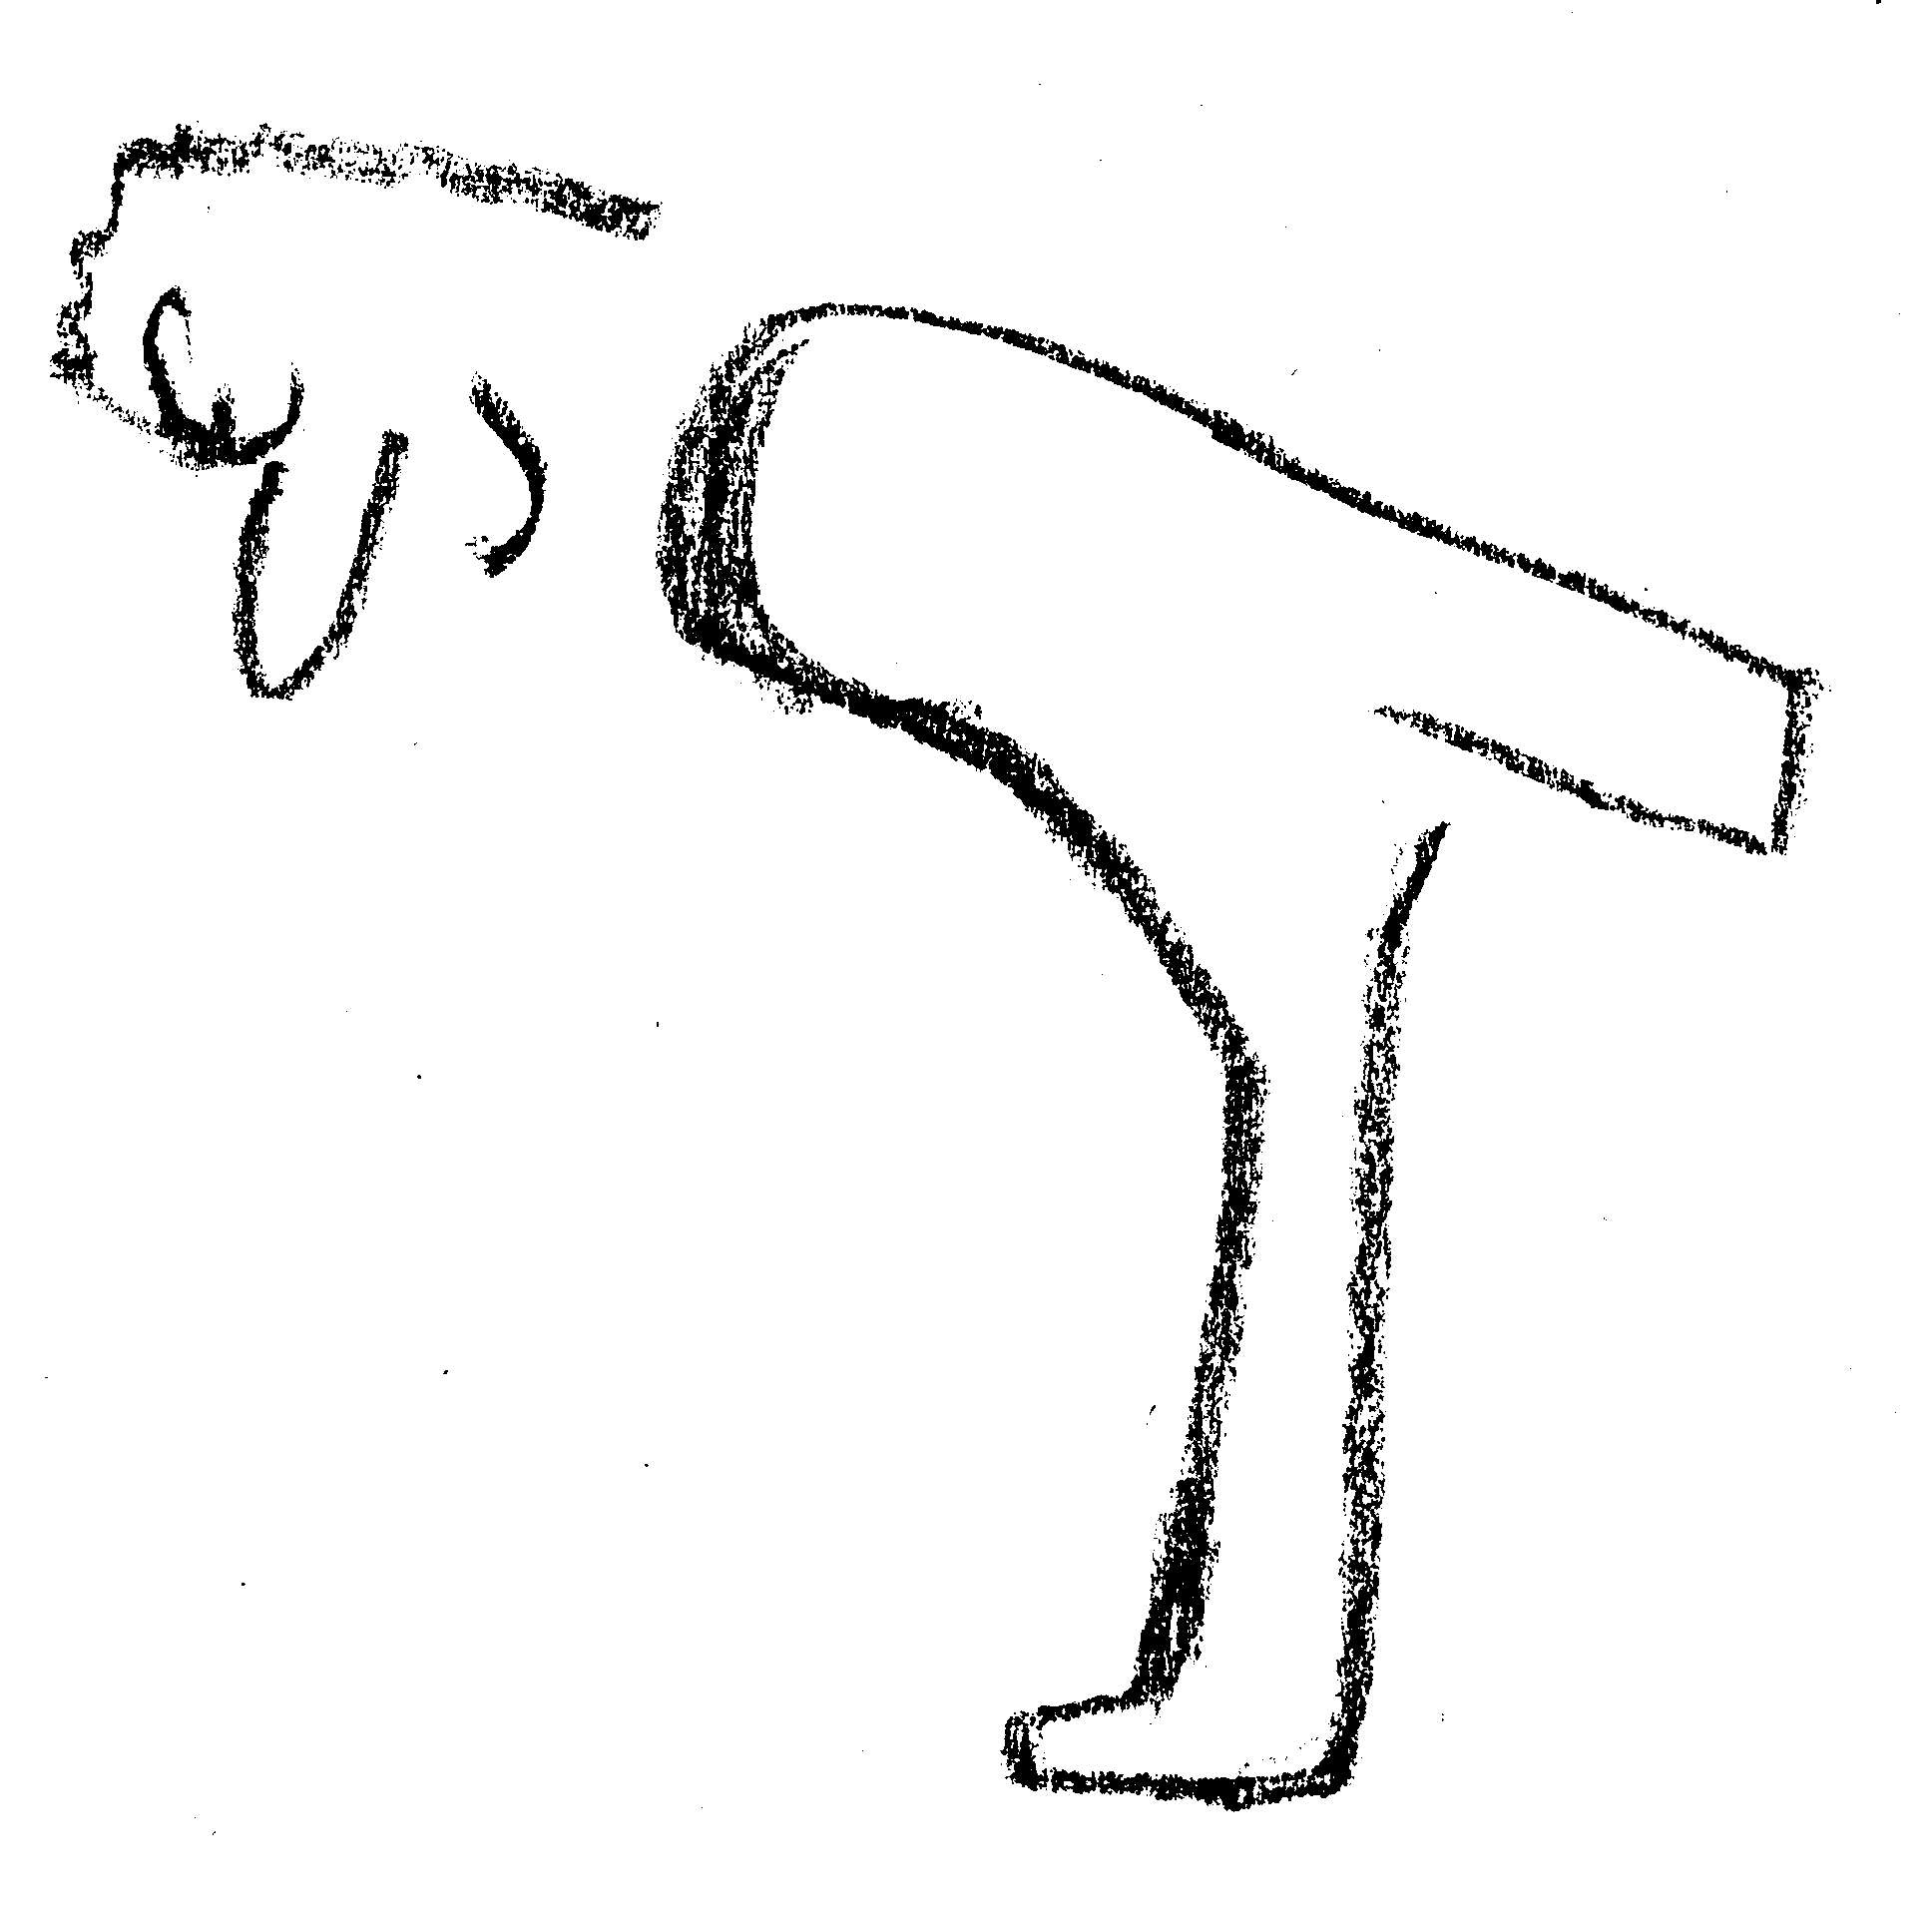
\includegraphics[width=.6\textwidth]{images/end}
   \end{column}
 \end{columns}
\end{frame}


\end{document}

